\section{Recurrence networks in phase space} \label{sec:RecurrenceNt}
In this section, we introduce and discuss recurrence networks (RNs) together with similar types of phase space based complex network representations of time series as an alternative framework for studying recurrences in phase space from a geometric point of view. We start with introducing the notion of a recurrence plot (RP) \cite{Eckmann1987,marwan2007}, which provides the fundamental framework for the visual and dynamical analysis of individual dynamical systems. Subsequently, different types of related network representations are introduced together with a detailed discussion of the resulting network characteristics of recurrence networks and their interpretation. In this context, we highlight the capability of these networks to unveil geometric characteristics associated with the structural organization of the underlying system in its phase space, which distinctively differs from other recurrence based techniques like recurrence quantification analysis (RQA) \cite{zbilut92,trulla96}, recurrence time statistics, or estimation of dynamical invariants from RPs. Finally, we close this section by introducing and discussing different bi- and multivariate generalizations of the recurrence network concepts and their respective interpretations, focusing on recent extensions of cross-recurrence plots \cite{marwan2002,Zbilut1998}, joint recurrence plots \cite{romano2004} and multiplex recurrence plots \cite{Eroglu2018}.


	\subsection{Theoretical background}
		\subsubsection{Phase space and attractor reconstruction} \label{sec:attractorReconstruct}
		We start with a (possibly multivariate) time series $\{x_i\}_{i=1}^N$ with $x_i=x(t_i)$, which we interpret as a finite representation of the trajectory of some (deterministic or stochastic) dynamical system. For a discrete system (map), the sampling of the time series is directly given by the map, whereas for a continuous-time system, the time series values correspond to a temporally discretized sampling of a finite part of one trajectory of the system determined by some initial conditions together with the corresponding sampling rate.

        In the case of observation functions not representing the full variety of dynamically relevant components, we additionally assume that attractor reconstruction has been performed \cite{Fraser1986,kantz1997,Kennel1992,Takens1981}. More specifically, when given a scalar time series $\{x_i\}$ ($i=1,\dots,N$), we first convert the data into state vectors in some appropriately reconstructed phase space. A common method from dynamical systems theory to define such a phase space is time-delay embedding~\cite{Takens1981}. In fact, the concept of a phase space representation rather than a ``simple'' time or frequency domain approach is the hallmark of many methods of nonlinear time series analysis, requiring embedding as the first step. Here, we define $\vec{x}_i = (x_i, x_{i-\tau}, \cdots, x_{i-(m-1)\tau})$ to obtain an $m$-dimensional time-delay embedding of $x_i$ with embedding delay $\tau$ for obtaining state vectors in phase space~\cite{Takens1981}. It has been proven that for deterministic dynamical systems, the thus reconstructed phase space is topologically equivalent to the original space if $m > 2 D_F$, where $D_F$ is the fractal dimension of the support of the invariant measure generated by the dynamics in the true (but often at most partially observed) state space. Note that $D_F$ can be much smaller than the dimension of the underlying original (physical) phase space spanned by all relevant system variables.

		From a practical perspective, when analyzing a scalar time series of whatever origin, neither embedding dimension $m$ nor delay $\tau$ are known a priori. The false nearest-neighbors (FNN) method~\cite{Kennel1992} was introduced to derive a reasonable guess of how to choose $m$ based on studying whether or not proximity relations between state vectors are lost when the embedding dimension is successively increased. If a reasonable embedding dimension is found, all dynamically relevant coordinates of the system are appropriately represented, so that all proximity relationships are correct and not due to lower-dimensional projection effects.

		In a similar spirit, a delay $\tau$ may be appropriate when the statistical dependence between the components of the embedding vector $\vec{x}$ approaches zero. For example, this can be achieved by choosing $\tau$ corresponding to the first root of the auto-correlation function (ACF) of a time series. This minimizes the linear correlation between the components, but does not necessarily mean they are independent. However, the converse is true: if two variables are statistically independent they will be uncorrelated. Therefore, another well established strategy for determining $\tau$ is to use the first minimum of the time-delayed mutual information \cite{Fraser1986}.

		The aforementioned approaches to determining $m$ and $\tau$ commonly work well for data from deterministic dynamical systems. It is an important issue when dealing with experimental time series and we have to first check if appropriate embeddings are applicable. Practically, we need to show the dependence of any analysis on the embedding explicitly. Let us first assume in the following sections that a proper embedding has been obtained, before discussing the possible effects of embedding parameters on the reconstructed recurrence networks in Section \ref{subsubsec:embedding}.

		\subsubsection{Recurrences and recurrence plots}
		Recurrence of states, in the meaning that states become again arbitrary close to previous ones after some time, is a fundamental property of deterministic dynamical systems and is typical for nonlinear or chaotic systems \cite{Ott1993,poincare1890}. From the set of (original or reconstructed) state vectors representing a discrete sampling of the underlying system's trajectory (e.g., the chaotic attractor of a dissipative system), recurrences can be visualized by recurrence plots (RP) \cite{marwan2007}, originally introduced by Eckmann {\textit{et al.}} \cite{Eckmann1987}. The RP is a graphical representation of the corresponding recurrence matrix $\textbf{R}(\varepsilon)$ that is defined in the standard way as
\begin{equation} \label{eq:rpDefinition}
R_{ij}(\varepsilon)=\Theta(\varepsilon-\|\vec{x}_i - \vec{x}_j\|),
\end{equation}
\noindent
where $\|\cdot\|$ can be any norm in phase space (e.g., Manhattan, Euclidean, or maximum norm). For convenience, we will use the maximum norm in all following examples unless stated otherwise. A RP enables us to investigate the recurrences of the $m$-dimensional phase space trajectory through a two-dimensional graphical representation $R_{ij}$ in terms of black and white dots indicating recurrent and non-recurrent pairs of vectors, respectively. The algorithmic parameter $\varepsilon$ is a pre-defined threshold value which determines whether two state vectors are close or not. The effects of $\varepsilon$ on the resulting RP and their statistics will be further discussed in Section \ref{subsub:epsilon}.

The basic principle of a RP is illustrated in Fig.~\ref{lorenz_constr} for one realization of the Lorenz system (Eq. \eqref{eqlorenz}). Further more specific alternative definitions of recurrences add dynamical aspects, such as local rank orders or strictly parallel evolution of states (parallel segments of phase-space trajectory considered in iso-directional RPs~\cite{Horai2002}). For a more detailed overview, we refer to~\cite{marwan2007}.
\begin{figure}
	\centering
	\includegraphics[width=\textwidth]{Chapter03_RecurrenceNt/lorenz_constr.eps}
\caption{Basic concepts beyond recurrence plots and the resulting recurrence networks (RNs), exemplified for one realization of the Lorenz system (Eq.~(\ref{eqlorenz})) using the same time series as in Fig. \ref{fig:lorenz_network}(e). (a) A state at time $i$ (red dot) is recurrent at another time $j$ (black dot) when the phase space trajectory visits its close neighborhood (gray circle). This is marked by value 1 in the recurrence matrix at $(i,j)$. States outside of this neighborhood (small open red circle) are marked with 0 in the recurrence matrix. (b) Graphical representation of the corresponding recurrence matrix (recurrence plot, Eq. \eqref{eq:rpDefinition}) and adjacency matrix of the RN (modulo main diagonal). (c) A particular path in the RN for the same system embedded in the corresponding phase space. Reproduced from \cite{Donner2011} with permission by World Scientific Publishing Co.. }
\label{lorenz_constr}
\end{figure}

RPs of dynamical systems with different types of dynamics exhibit distinct structural properties, which can be characterized in terms of their associated small-, medium- as well as large-scale features~\cite{marwan2007}. The study of recurrences by means of RPs has become popular with the introduction of recurrence quantification analysis (RQA)~\cite{zbilut92,marwan2002herz}. The initial purpose of this framework has been to introduce measures of complexity which distinguish between different appearances of RPs~\cite{marwan2008epjst}, since they are linked to certain dynamical properties of the studied system. RQA measures use the distribution of small-scale features in the RP, namely individual recurrence points as well as diagonal and vertical line structures. For instance, the recurrence rate (RR) simply counts the density of recurrence points of the matrix $\textbf{R}(\varepsilon)$ for a given threshold $\varepsilon$ (Eq.~\eqref{eq:rpDefinition}). RQA as a whole has been proven to constitute a very powerful technique for quantifying differences in the dynamics of complex systems and has meanwhile found numerous applications, e.g., in ecology \cite{facchini2007}, engineering \cite{litak2009c}, geo- and life sciences \cite{marwan2003climdyn,marwan2007pla}, or protein research \cite{Giuliani2002a,zbilut2004a}.  For a more comprehensive review on the potentials of this method, we refer to \cite{marwan2007,marwan2008epjst,webber2009}. In addition, we would like to remark that even dynamical invariants, like the $K_2$ entropy, mutual information, or fractal dimensions (i.e., the information and correlation dimensions $D_1$, $D_2$) can be efficiently estimated from RPs \cite{thiel2004a,marwan2007}. Moreover, RPs have also been successfully applied to study interrelations, couplings, and phase synchronization between dynamical systems~\cite{marwan2002,romano2004,romano2005,Romano2007,vanLeeuwen2009,Nawrath2010,marwan2013c}.

In order to highlight different domains of recurrences in the RPs, some algorithms have been proposed recently. For example, Pham {\textit{et al.}} introduced fuzzy recurrence plots, which determine an optimal relation between the observed states in phase space and a number of predefined clusters \cite{Pham2016}. This algorithm highlights the recurrence regions and, thus, provides possibly clearer visualization of the underlying recurrence structures. An alternative algorithm has been proposed in \cite{graben2013} to search for specific recurrence domains. Here, intersecting $\varepsilon$-balls around sampling points are merged into cells of a phase space partition, and a maximum entropy principle defines the optimal size of these intersecting balls. This data-adaptive algorithm for obtaining phase partitions has been found to perform better than techniques based on Markov chains, which require an ad hoc partition of the system's phase space. Along the same lines of research, another algorithm has been proposed recently in \cite{Costa2018} to capture the recurrence density structures in the RP.


	\subsection{Types of recurrence networks}
		\subsubsection{$\varepsilon$-recurrence networks}
		The crucial step of the recurrence network approach is to re-interpret the mathematical structure $\textbf{R}(\varepsilon)$ as the adjacency matrix $\mathbf{A}$ of some adjoint complex network embedded in phase space by setting
\begin{equation}
\mathbf{A}(\varepsilon)=\mathbf{R}(\varepsilon)-\mathbf{1}_N,
\label{eq:rn_definition}
\end{equation}
\noindent
where $\mathbf{1}_N$ is the $N$-dimensional identity matrix. The complex network defined this way is called \emph{$\varepsilon$-recurrence network (RN)}, as opposed to other types of proximity-based networks in phase space making use of different definitions of geometric closeness, e.g., considering $k$-nearest neighbors~\cite{Donner2011}, which will be further discussed below. Specifically, the sampled state vectors $\{x_i\}$ are interpreted as vertices of a complex network, which are connected by undirected edges if they are mutually close in phase space (i.e., describe recurrences). In the remainder of this review, we will adopt the time indices $i$, $j$, etc., of observations as vertex indices of the corresponding time series networks to highlight their equivalence whenever individual observations or state vectors coincide one-by-one with the vertices of the network representations (which is the case for recurrence networks, but also visibility graphs and related methods discussed later in this review). Notably, the binary matrix $\mathbf{A}(\varepsilon)$ retains the symmetry properties of $\mathbf{R}(\varepsilon)$, which implies that the RN is a \emph{simple graph}, i.e., a complex network without multiple edges or self-loops (note that $A_{ii}=0$ according to definition~(\ref{eq:rn_definition})). We show an example of such an unweighted  $\varepsilon$-RN network in Fig. \ref{lorenz_net}.
\begin{figure}
	\centering
	\includegraphics[width=0.48\textwidth]{Chapter03_RecurrenceNt/lorenz_net.eps}
\caption{A graphical representation of the Lorenz attractor based on the recurrence matrix represented in Fig.~\ref{lorenz_constr}. The color of the vertices corresponds to their temporal order (from orange to bright green). Reproduced from \cite{Donner2011} with permission by World Scientific Publishing Co.. }
\label{lorenz_net}
\end{figure}

		One of the fundamental concepts of network theory is the notion of a {\textit{path}} (Section \ref{sec:basicCompNets}). In an $\varepsilon$-RN, a \emph{path} between two specified vertices $i$ and $j$ is an ordered sequence of edges starting at $i$ and ending at $j$, with its \emph{path length} $l_{ij}(\varepsilon)$ given by the number of edges in this sequence. An example of a path is shown in Fig. \ref{lorenz_constr}(c). In the context of RNs, we can thus understand a path as a sequence of mutually overlapping $\varepsilon$-balls $B_{\varepsilon}(x_i),B_{\varepsilon}(x_{k_1}),\dots,B_{\varepsilon}(x_{k_{l_{i,j}-1}}),B_{\varepsilon}(x_j)$, where $$B_{\varepsilon}(x)=\{y\,|\,\|x-y\|<\varepsilon\}$$ is an open set describing a volume with maximum distance $\varepsilon$ (measured in a given norm) from $x$, and $B_{\varepsilon}(x_i)\cap B_{\varepsilon}(x_{k_1})\neq\emptyset,\dots,B_{\varepsilon}(x_{k_{l_{i,j}-1}})\cap B_{\varepsilon}(x_j)\neq\emptyset$. Note that $\varepsilon$-balls refer to general (hyper-)volumes according to the specific norm chosen for measuring distances in phase space, e.g., hypercubes of edge length $2 \varepsilon$ in case of the maximum norm, or hyperballs of radius $\varepsilon$ for the Euclidean norm.

		Following these considerations, a \emph{shortest path} is a minimum sequence of edges (connecting vertices in mutually overlapping $\varepsilon$-balls) between two fixed vertices (state vectors) $i$ and $j$. Note that a shortest path does not need to be unique. In turn, due to the discrete character of a network, it is rather typical that there are multiple shortest paths between some specific pair of vertices. In what follows, the shortest path length will be denoted as ${l}_{ij}$, and the multiplicity of such shortest paths as ${\sigma}_{ij}$, following the corresponding general notation introduced in Section~\ref{sec:CompNetworkT}.

		We have to emphasize that the network-theoretic concept of a path on a given graph is distinctively different from the trajectory concept that records the dynamical evolution of a system \cite{Donner2010a}. Furthermore, RNs based on Eq.~(\ref{eq:rn_definition}) can be generalized by withdrawing the application of a specific threshold, which leads to weighted networks and unthresholded RPs (distance plots), respectively. For example, the unthresholded RP obtained from one trajectory of a given dynamical system may be re-interpreted as the connectivity matrix of a fully coupled, weighted network in phase space.

	 	Most of RN analysis has focused on the network representation using the adjacency matrix $\mathbf{A}(\varepsilon)$ (Eq.~\eqref{eq:rn_definition}) and the extraction of new network-theoretic measures, which will be reviewed below. We emphasize that $\mathbf{A}(\varepsilon)$ provides information on vertices and edges, but its graph structural layouts can take variable forms.  Network visualization is a non-trivial task and there are many tools for that purpose in computer science, e.g., spring-based layout systems, spectral layout method, tree layout algorithms, etc. These algorithms have been well integrated in many popular network visualization packages, i.e., \texttt{Mathematica}, \texttt{Gephi}, and \texttt{NetworkX}. The network visualization shown in Fig.~\ref{lorenz_net} has been created by the software package {\tt{GUESS}} using a force-directed placement algorithm. In \cite{Yang2013}, Yang {\textit{et al.}} proposed to use a spring-electrical model to explore the self-organized geometry of RNs. In this algorithm, they simulate the recurrence network as a physical system by treating the edges as springs and the nodes as electrically charged particles. Then, force-directed node placement algorithms are employed to automatically organize the network geometry by minimizing the system energy. It has been shown that this self-organized process recovers the attractor of a dynamical system, which provides important insights for attractor reconstruction from the adjacency matrix \cite{thiel2004b,hirata2008}.


		\subsubsection{$k$-nearest neighbor networks}
		Besides the recurrence definition based on a fixed distance threshold $\varepsilon$ in phase space (i.e., equal neighborhood volumes around all available state vectors), there are alternative ways for defining recurrences and, hence, RPs and RNs. For example, the original definition of a RP by Eckmann \textit{et~al.} \cite{Eckmann1987} makes use of $k$-nearest neighbors (i.e., a fixed probability mass of the considered neighborhoods). Re-interpreting the resulting recurrence matrix as the adjacency matrix of a complex network leads to a different type of RN \cite{Shimada2008}, typically referred to as \emph{$k$-nearest neighbor network}. Since in this definition, the neighborhood relation is not symmetric (i.e., $x_j$ being among the $k$ nearest neighbors of $x_i$ does not imply $x_i$ also being among the $k$ nearest neighbors of $x_j$), the resulting networks are in general directed graphs, and the local density of unidirectional edges (as opposed to bidirectional ones) is related to the gradient of the invariant density.

		\subsubsection{Adaptive neighbor networks} \label{sec:adaptiveRN}
		In order to circumvent the directedness of $k$-nearest neighbor networks, Xu \textit{et~al.} \cite{Small2009,Xu2008} proposed an algorithm for balancing the neighborhood relationships in such a way that they become symmetric again. The resulting networks embedded in phase space, sometimes also referred to as \emph{adaptive nearest neighbor networks} \cite{Donner2011}, are conceptually more similar to classical ($\varepsilon$-)RNs, but still exhibit somewhat different topological characteristics. In particular, this approach helps to understand the superfamily phenomena of time series, which concern the relative prevalence of motifs of the resulting networks. In particular, the motif distribution of adaptive nearest neighbor networks has been empirically shown to allow a discrimination between different types of dynamics in terms of a different motif ranking \cite{Xu2008}. Consequently, this approach has been mainly used for such discriminatory tasks, including applications to turbulence phenomena, instrumental music \cite{Donner2011}, fractional Brownian motions and multifractal random walks \cite{Liu2010a}.

		While these superfamily phenomena have been found in time series from various origins, no fundamental theories have been proposed so far in the literature to explain the corresponding empirical findings. Khol {\textit{et al.}} provide a heuristic explanation of superfamily phenomena by examining the dependence of the attractor dimension on motif prevalence \cite{Khor2016}. Since the constructed networks inherently capture the proximity of states, motifs represent specific arrangements of states in space, some of which are more or less likely to occur as dimension changes. Therefore, they found that the relative prevalence of motifs is strongly dependent on the local dimension of the space from which the state vectors are taken. Further evidence is given by identifying comparable superfamily phenomena in networks constructed from states randomly distributed in spaces of varying dimensions \cite{Khor2016}.

		\subsubsection{Algorithmic variants}
		A detailed discussion of the differences between $\varepsilon$-RNs, $k$-nearest neighbor and adaptive nearest neighbor networks introduced above has been recently provided in \cite{Donner2011}. While these three classes of time series networks exhibit very strong conceptual similarities (the same applies to the correlation networks \cite{Yang2008} discussed in Section~\ref{sec:correlationnetworks} if interpreting the correlation coefficient between two sufficiently high-dimensional state vectors as a generalized distance), the approach proposed by Li \textit{et~al.} \cite{Li2011a,Li2011b,Cao2014,Fan2015} can be understood as being derived from the RN idea. Here, for a set of $m$-dimensional embedding vectors, all mutual Euclidean distances are computed. Based on the maximum distance value $d_{max}(m)$, the threshold distance of a RN is taken as $\varepsilon(m)=d_{max}(m)/(N-1)$. This procedure is repeated for different $m$, and the critical value of the embedding dimension for which the resulting network gets completely disconnected is interpreted as a complexity index \cite{Cao2014}. However, it has not yet been demonstrated that this algorithmic approach has any conceptual benefits in comparison with the classical RN measures like transitivity (see Section~\ref{sec:transitivity}) obtained for a fixed embedding dimension. Moreover, we note that the maximum distance $d_{max}$ between embedding vectors may depend on the embedding dimension in some peculiar form, e.g., may be independent for the supremum norm while increasing monotonically for most other common norms \cite{Kraemer2018}. In this regard, it is commonly recommended to study fixed quantiles of the distance distribution function rather than fixed multiples of some location parameters (like mean, median or maximum) of the latter \cite{Kraemer2018}.

		Another conceptual approach loosely related to RNs provides the foundation of the frequency-degree mapping algorithm introduced by Li \textit{et~al.} \cite{Li2012}. Here, the resulting time series networks contain two types of edges: (i) temporal edges connecting subsequent points in time, and (ii) proximity edges containing observations of similar values, where similarity is defined by an initial grouping of the data into a discrete set of classes, and observed values being connected if and only if they belong to the same class. Note that this is conceptually related to the idea of coarse-graining based transition networks that will be discussed in Section~\ref{sec:cgtn}. Here the definition of a class is equivalent to a recurrence interval that is defined by amplitude quantization, for instance, the recurrence interval length $I = H/Q$ where $Q$ is the quantization level and $H$ is the amplitude range of the time series. Notably, the latter approach combines the classical recurrence idea and basic concepts of symbolic dynamics \cite{Daw2003} (see Section~\ref{sec:symbolic}). In this spirit, the resulting network's adjacency matrix is given as the recurrence matrix associated with a symbolic recurrence plot \cite{Donner2008,Faure2010,graben2013} plus a ``stripe'' around the matrix' main diagonal. The frequency-degree mapping algorithm has been successfully applied to characterizing signatures of various types of ventricular arrhytmias in human heart beat time series \cite{Li2012}, stock markets \cite{Cao2014}, and air quality indices \cite{Fan2015}.

		In order to highlight the recurrence domains in networks, the fuzzy recurrence network approach has been proposed in \cite{Pham2017}, which shares many similarities with fuzzy recurrence plots \cite{Pham2016}. Furthermore, a grammatical rewriting algorithm over the recurrence matrix has been proposed to search for recurrence domains in \cite{graben2013}, which presents a symbolic description of the recurrence properties of a time series. It is interesting to see that this algorithm yields an optimal symbolic recurrence representation revealing functional components of brain signals \cite{graben2013}. Note that the computation of the recurrence matrix is the first step of this grammatical algorithm.

		The computation time of a RN is proportional to $N^2$ where $N$ is the number of time points, which calls for more efficient algorithms for constructing RNs for long time series. In this case, on the other hand, we are more interested in the evolution of the RN over time. To this end, sliding window techniques are often suggested but require checking the dependence of the corresponding results on the window size \cite{Donges2011a,Donges2011}. Another idea is to perform coarse graining of the original RNs \cite{Costa2018}, which originates from the idea of meta-recurrence plots \cite{casdagli97}. In \cite{Iwayama2012}, the authors proposed to first divide the original long time series into short segments and RNs are then constructed for each piece. The next step is to build joint recurrence networks for each pair of windowed segments. Then, the long-term dynamics is characterized by the variations of the network properties computed for these meta-time series.


		\subsection{Complex network characteristics of RN} \label{sec:rn_measures}
		Based on the re-interpretation of the recurrence matrix $\mathbf{R}(\varepsilon)$ as the adjacency matrix of an adjoint RN, we can utilize the large toolbox of complex network measures (see Section~\ref{sec:basictheoryCN})~\cite{Albert2002,Boccaletti2006,Costa2007,Newman2003} for characterizing the structural organization of a dynamical system in its phase space. Notably, this viewpoint is complementary to other concepts of nonlinear time series analysis making use of RPs. For example, RQA characterizes the statistical properties of line structures in the RP, which implies an explicit consideration of dynamical aspects (i.e., sequences of state vectors) \cite{marwan2007}. In turn, RNs do not make use of time information, since network properties are generally invariant under vertex relabelling (i.e., permutations of the order of observations) \cite{Donner2010a}. In this spirit, RN analysis provides geometric instead of dynamical characteristics. This idea of a geometric analysis is similar to some classical concepts of fractal dimensions (e.g., box-counting or correlation dimensions), where certain scaling laws in dependence on the spatial scale of resolution (corresponding here to $\varepsilon$) are exploited. In turn, RN analysis can be performed (as RQA) using only a single fixed scale ($\varepsilon$) instead of explicitly studying scaling properties over a range of threshold values. We will further elaborate on this idea in Section~\ref{sec:transitivity}.

		The distinction between dynamical and geometric information implies that in case of RN analysis, the typical requirement of a reasonable (typically uniform) temporal sampling of the considered trajectory is replaced by the demand for a suitable spatial coverage of the system's attractor in phase space. Specifically, under certain conditions the latter could also be obtained by considering an ensemble of short trajectories instead of a single long one. If the trajectory under study is relatively densely sampled, trivial serial correlations can lead to a selection bias in the set of sampled state vectors; the latter could be avoided by reasonable downsampling. In the same context, the possibility of utilizing Theiler windows for removing edges representing short-term auto-correlations (e.g., recurrence points close to the main diagonal in the RP) should be mentioned as another strategy based on a somewhat different rationale~\cite{Donner2010a}. However, from a conceptual perspective, downsampling can provide an unbiased sampling of the attractor as long as the fixed sampling time does not correspond to any integer multiple of some of the system's natural frequencies. As an alternative, bootstrapping from the set of available state vectors provides another feasible option, which should be preferred if a sufficiently long time series is available. In general, numerical experiments and different applications suggest that stable estimates of RN characteristics can often already be obtained using a sample size of $N\sim\mathcal{O}(10^2\dots 10^3)$ data points~\cite{Donges2011,Donges2011a}.

		In Section~\ref{sec:basictheoryCN}, we have provided a general review on various network measures characterizing the structural properties of a complex network as denoted by the adjacency matrix $\mathbf{A}$. In this section, we further discuss the physical interpretations of these measures in terms of phase space properties as captured by RN representations. In what follows, we will denote some basic properties computed from a RN consisting of a finite number $N$ of state vectors as $\hat{f}$, pointing to the fact that they are estimated from a given sample of state vectors but shall characterize the entire trajectory of the system under study. In other words, we have specific finite sample estimates for Eqs.~\eqref{eq:degree}-\eqref{eq:apl}. Furthermore, we will discuss a corresponding continuous framework describing all network characteristics described below in terms of some fully analytical theory in Section \ref{sec:analyticRNtheory}. In order to focus the following discussion, we review only the possibly most relevant characteristics associated with RNs. More details including further measures can be found in \cite{Donges2012,Donner2010a}.

		When considering the quantitative characteristics of complex networks (see Section~\ref{sec:basictheoryCN}), different classifications of measures are possible \cite{Donner2010a,Donges2012}. First, we may distinguish measures based on the concept of graph neighborhoods from those making use of shortest path-based characteristics. This is not an exhaustive classification, since it potentially neglects other important network measures, e.g., such based on diffusion processes or random walks on the network. Second, network measures can be classified into such making use of local, meso-scale and global information. This scheme is widely equivalent to the first one in that local information refers to properties determined by the graph neighborhood of a given vertex, whereas global information takes contributions due to all vertices of the network into account, which is common for shortest path-based measures. Finally, we can differentiate between measures quantifying properties of single vertices, pairs of vertices, and the network as a whole. In the following, we will utilize the latter way of classification, since it appears most instructive from the applied point of view (i.e., we are commonly interested in either the local or the global geometry of an attractor or, more generally, some trajectory in phase space). Furthermore, we emphasize that in practice, the phase space properties captured by the estimates of RN characteristics are obtained for a particular value of $\varepsilon$. The effects of varying $\varepsilon$ on the resulting network statistics will be further discussed in Section \ref{subsub:epsilon}.

        In the following, we will adopt the notation of indexing each vertex of a RN with the time index $i$ (respectively, $j$, $k$, etc.) of the corresponding state vector $\vec{x}_i$ (etc.) instead of using the general vertex indices $p$, $q$, $r$, $s$, etc.\, used in Section~\ref{sec:basictheoryCN}. From here onward, we will adopt this notation whenever vertices can be uniquely identified with a point in time (respectively, the corresponding state or reconstructed state vector), which will also apply to the visibility graph based methods to be discussed in Section~\ref{sec:VisibilityGt}, but typically not to the transition networks reviewed in Section~\ref{sec:TransitionNt}. Moreover, some other types of proximity networks like cycle networks and correlation networks, which will be introduced in Section~\ref{sec:otherproxnets}, do not allow a unique identification of individual states (state vectors) with specific nodes of the networks, so that we will also adopt the more general index notation there.

			\subsubsection{Vertex characteristics}
        			From the perspective of recurrences, it is reasonable to replace the degree $\hat{k}_i(\varepsilon)$ (Eq.~\ref{eq:degree}) of a vertex by a normalized characteristic, the \textit{degree density} $\hat{\rho}_i(\varepsilon) =\frac{\hat{k}_i(\varepsilon)}{N-1}$, which corresponds to the definition of the local recurrence rate of the state $\vec{x}_i$. This means that $\hat{\rho}_i(\varepsilon)$ quantifies the density of states in the $\varepsilon$-ball around $\vec{x}_i$, i.e., the probability that a randomly chosen member of the available sample of state vectors is $\varepsilon$-close to $x_v$. An illustration of this fact for the Lorenz system is presented in Fig.~\ref{fig:local}(a); here, phase space regions with a high density of points (i.e., a high residence probability of the sampled trajectory) are characterized by a high degree density.
\begin{figure}
	\centering
	\includegraphics[width=\columnwidth]{Chapter03_RecurrenceNt/phase_deg_cc_cls_btwLoenz.eps}
\caption{Spatial distributions of vertex characteristics of the $\varepsilon$-RN obtained for the Lorenz system (Eq.~\ref{eqlorenz}) at the canonical parameters (using the maximum norm with $\hat{\rho}=0.01$, $N=20,000$ and sampling time $\Delta t=0.1$): (a) $\hat{k}_i(\varepsilon)$, (b) $\hat{\mathcal{C}}_i(\varepsilon)$, (c) $\hat{c}_i(\varepsilon)$, (d) $\hat{b}_i(\varepsilon)$. Modified from \cite{Donner2010a}. } \label{fig:local}
\end{figure}

			The \textit{local clustering coefficient} (Eq.~\ref{eq:locclustering}) $\hat{\mathcal{C}}_i(\varepsilon)$ measures the fraction of pairs of vertices in the $\varepsilon$-ball around $\vec{x}_i$ that are mutually $\varepsilon$-close. For vertices with $\hat{k}_i(\varepsilon)<2$, we define $\hat{\mathcal{C}}_i(\varepsilon)=0$. It has been shown that the local clustering coefficient in a RN is associated with the geometric alignment of state vectors. Specifically, close to dynamically invariant objects such as unstable periodic orbits (UPOs) of low period, the dynamics of the system is effectively lower-dimensional, which results in a locally enhanced fraction of closed paths of length 3 (``triangles'') and, thus, a higher local clustering coefficient. The latter behavior is exemplified in Fig.~\ref{fig:local}(b) for the Lorenz system, where we recognize certain bands with higher values of $\hat{\mathcal{C}}_i$ corresponding to the positions of known low-periodic UPOs~\cite{Donner2010a}. The deeper reasons for this behavior will be further addressed in Section~\ref{sec:transitivity}.

			For estimating the \textit{closeness} (Eq.~\ref{eq:closeness}) $\hat{c}_i(\varepsilon)$ and \textit{local efficiency} (Eq.~\ref{eq:locefficiency}) $\hat{e}_i(\varepsilon)$, we again set $\hat{d}_{ij}$ to the highest possible value of $N-1$ for pairs of vertices that cannot be mutually reached. Both measures exhibit the highest values for vertices which are situated in the center of the RN (see Fig.~\ref{fig:local}(c) for an illustration for the Lorenz system).

			The \textit{betweenness} (Eq.~\ref{eq:betweenness}) $\hat{b}_i(\varepsilon)$ of nodes in a RN can be interpreted as indicating the local degree of fragmentation of the underlying attractor~\cite{Donner2010a}. To see this, consider two densely populated regions of phase space that are separated by a poorly populated one. Vertices in the latter will ``bundle'' the shortest paths between vertices in the former ones, thus forming geometric bottlenecks in the RN. In this spirit, we may understand the spatial distribution of betweenness centrality for the Lorenz system (Fig.~\ref{fig:local}(d)) which includes certain bands with higher and lower residence probability reflected in lower and higher betweenness values.

  		\subsubsection{Edge characteristics}
		The \textit{matching index} (Eq.~\ref{eq:matching}) $\hat{m}_{ij}(\varepsilon)$ quantifies the overlap of the network neighborhoods of two vertices $i$ and $j$. From the above definition, it follows that $\hat{m}_{ij}(\varepsilon)=0$ if $\|\vec{x}_i-\vec{x}_j\|\geq 2\varepsilon$. In turn, there can be mutually unconnected vertices $i$ and $j$ ($A_{ij}=0$) with $\varepsilon\leq \|\vec{x}_i-\vec{x}_j\|< 2\varepsilon$ that have some common neighbors and, thus, non-zero matching index. In the context of recurrences in phase space, $\hat{m}_{ij}(\varepsilon)=1$ implies that the states $\vec{x}_i$ and $\vec{x}_j$ are twins, i.e., share the same neighborhood in phase space \cite{thiel2006b}. In this spirit, we interpret $\hat{m}_{ij}(\varepsilon)$ measures the degree of twinness of two state vectors. Note that twins have important applications in creating surrogates for testing for the presence of complex synchronization~\cite{thiel2006b,Romano2009}.

		As the node betweenness of a RN, the associated \textit{edge betweenness} (Eq.~\ref{eq:edgebetweenness}) $\hat{b}_{ij}(\varepsilon)$ characterizes the local fragmentation of the studied dynamical system in its phase space.

		For the specific case of $\varepsilon$-RNs, we emphasize that there is no simple correspondence between matching index and edge betweenness, since both quantify distinctively different aspects of phase space geometry. Specifically, there are more pairs of vertices with non-zero matching index than edges, even though there are also pairs of vertices with $\hat{b}_{ij}(\varepsilon)>0$ but $\hat{m}_{ij}(\varepsilon)=0$ (i.e., there is an edge between $i$ and $j$, but both have no common neighbors). However, for those pairs of vertices for which both characteristics are non-zero, we find a clear anti-correlation \cite{Donner2010a}. One interpretation of this finding is that a large matching index typically corresponds to very close states in phase space; such pairs of RN vertices can in turn be easily exchanged as members of shortest paths on the network, which implies lower edge betweenness values. A similar argument may explain the coincidence between high edge betweenness and low non-zero matching index values.

		\subsubsection{Global network characteristics} \label{subsubsec:RNmeasureG}
		The \textit{edge density} (Eq.~\ref{eq:edgedensity}) $\hat{\rho}(\varepsilon)$. Notably, for a RN the edge density equals the recurrence rate $RR(\varepsilon)$ of the underlying RP. Strictly speaking, this is only true if the recurrence rate is defined such as the main diagonal in the RP is excluded in the same way as potential self-loops from the RN's adjacency matrix. It is trivial to show that $\hat{\rho}(\varepsilon)$ is a monotonically increasing function of the recurrence threshold $\varepsilon$: the larger the threshold, the more neighbors can be found, and the higher the edge density.

		The arithmetic mean of the local clustering coefficients $\hat{\mathcal{C}}_i(\varepsilon)$ of all vertices $i$ (Eq.~\ref{eq:globclustering}) defines the \emph{global clustering coefficient} $\hat{\mathcal{C}}(\varepsilon)$ in the usual way (see Section~\ref{sec:basictheoryCN}). Given our interpretation of the local clustering coefficient in a RN, $\hat{\mathcal{C}}(\varepsilon)$ can be interpreted as a proxy for the average local dimensionality of the dynamical system in phase space. Analogously, the \textit{network transitivity} (Eq.~\ref{eq:transitivity}) $\hat{\mathcal{T}}(\varepsilon)$ characterizes the effective global dimensionality of the system. In Section~\ref{sec:transitivity}, we will further expand this discussion by introducing the corresponding concepts of clustering and transitivity dimensions.

		The average path length (Eq.~\ref{eq:apl}) $\hat{\mathcal{L}}$ exhibits an inverse relationship with the recurrence threshold, since it approximates (constant) distances in phase space in units of $\varepsilon$~\cite{Donner2010a}. More specifically, the average phase space separation of states $\left<d_{ij}\right>$ serves as an $\varepsilon$-lower bound to $\hat{\mathcal{L}}$, namely,
\begin{equation}
\left<d_{ij}\right> \leq \varepsilon \hat{\mathcal{L}}. \label{avgL_eq}
\end{equation}
Interpreted geometrically, this inequality holds because $\hat{\mathcal{L}}$ approximates the average distance of states along geodesics on the RN (which can be considered as the geometric backbone of the attractor) in multiples of $\varepsilon$, while $\left<d_{ij}\right>$ gives the mean distance of states in $\mathbb{R}^m(\varepsilon)$ as measured by the norm $\|\cdot\|$.

	\subsection{Analytical theory of RN} \label{sec:analyticRNtheory}

	As we will demonstrate in the following, the properties of RNs can be also described analytically supporting their better understanding and, hence, applicability. For this purpose, we can exploit the formal equivalence of RNs and random geometric graphs (RGGs), a well-studied concept in graph theory and computational geometry. In this section, we motivate this equivalence and demonstrate how the variety of RN characteristics can be reformulated in the continuum limit $N\to\infty$ for any finite $\varepsilon$ \cite{Donges2012}. This framework allows gaining deep insights into the geometric organization of chaotic attractors by exploring the multitude of characteristics provided by complex network theory. Moreover, these analytical considerations will be extended to inter-system recurrence networks in Section \ref{sec:IntSRN}.


		\subsubsection{Preliminaries: random geometric graphs}
		Random geometric graphs \cite{Penrose2003} are based on a (finite) set of vertices randomly positioned in a $d$-dimensional ($d\in\mathbb{N}^+$) metric space according to some probability density function $p(\vec{x})$. In general, the connectivity among this set of vertices is taken to be distance-dependent, i.e., for two vertices $i$ and $j$, the probability of being connected in the RGG has the form $P(A_{ij}=1)=f(\|\vec{x}_i-\vec{x}_j\|)$ with some predefined function $f$, which is monotonically decreasing. As a consequence, spatially close vertices are more likely to be connected than distant ones. A particularly well studied special case is $f(\delta)=\Theta(\varepsilon-\delta)$ ($\delta$ denoting here the distance between any two points in the considered metric space as in Eq.~\eqref{eq:rpDefinition}), often referred to as RGG (in the strict sense). Notably, the latter definition has fundamental real-world importance (e.g., in terms of ad-hoc communication networks or, more general, contact networks) and matches that of the adjacency matrix of a RN (Eq.~\ref{eq:rn_definition}) if we identify $p(\vec{x})$ with the invariant density of the phase space object under study (e.g., some attractor in case of a dissipative system), and take the space in which the RGG is embedded as that spanned by the respective dynamical variables of the system. In this respect, for all following considerations, it is sufficient to restrict our attention to the support of $p(\vec{x})$ (respectively its closure), which is described by some manifold $S=\overline{\mbox{supp}(p)}$ embedded in the considered metric space (e.g., the attractor manifold).

		From a practical perspective, the spatial coverage of $p(\vec{x})$ by the RGG's vertices can be strongly affected by the sampling, leading to a spatial clustering of vertices if the sampling frequency is close to an integer multiple of the chaotic attractor's characteristic frequency. In such a situation, it is advantageous to follow alternative sampling strategies for $p(\vec{x})$. Note that for ergodic systems, sampling from one long trajectory, ensembles of short independent realizations of the same system, or directly from the invariant density should lead to networks with the same properties at sufficiently large $N$. In practice, generating the RGG/RN representation based on bootstrapping from the ensemble of available state vectors is often to be preferred over a regular sampling of a given trajectory, as discussed in Section~\ref{sec:rn_measures}.

		As outlined above, the importance of RGGs for the considerations on RNs is that some of their properties (like the degree distribution~\cite{Herrmann2003} or transitivity~\cite{Dall2002}) have been intensively studied for the generic case of a hard distance threshold in $f$ and arbitrary probability density functions $p(\vec{x})$ for metric spaces of various integer dimensions. For example, Hermann \textit{et~al.} \cite{Herrmann2003} give a closed-form expression of the degree distribution for arbitrary $p(\vec{x})$, whereas Dall and Christensen~\cite{Dall2002} provide a deep discussion of the transitivity properties of RGGs. Notably, the latter aspect has become particularly relevant in the interpretation of RN properties (see Section~\ref{sec:transitivity}) as well as those of some of their multivariate generalizations, as will be further discussed in Section~\ref{sec:IntSRN}.


		\subsubsection{Analytical description of $\varepsilon$-recurrence networks}
		By making use of the fact that RNs are a specific type of RGGs, all relevant graph-theoretical measures for RNs can be seen as discrete approximations of more general and continuous geometric properties of a dynamical system's underlying attractor characterized by a set $S$ together with an associated invariant density $p(\vec{x})$, $\vec{x}\in S$. This point of view allows obtaining deeper insights into the geometric meaning of the network quantifiers introduced in Section~\ref{sec:rn_measures} and enables us to establish surprising connections to other fields, e.g., the close relationship of transitivity measures like the local clustering coefficient and transitivity to the local and global fractal dimension of the dynamical system's attractor, respectively~\cite{Donner2011b} (see Section~\ref{sec:transitivity}). In the following, we review a corresponding analytical framework for general spatially embedded networks which is specifically tailored for defining continuous variants of the common discrete complex network characteristics \cite{Donges2012}.


		\paragraph{General setting}
		Let $S$ be a compact and smooth manifold with a non-vanishing continuous probability density function $p:S\to(0,\infty)$ with $\int_S d\vec{x}\ p(\vec{x}) = 1$. For the purpose of the present work, we identify $S$ with the set of points defining the attractor of a (dissipative) dynamical system. In case of chaotic attractors in time-continuous systems, we obtain a closure of the open attractive set by considering its union with the set of (infinitely many) unstable periodic orbits embedded in the attractor.

		Continuous analogs of the discrete complex network characteristics introduced in Section~\ref{sec:rn_measures} should be approximated by taking the limit $N\to\infty$ and $\varepsilon\to 0$ (note that the latter limit may not be assessible in the case of fractal sets $S$, which we will not further consider in the following). Here, ``continuous'' refers to a network with uncountably many vertices and edges, which is determined by the \emph{adjacency function}
\begin{equation}
A(\vec{x},\vec{y})=\Theta(\varepsilon-\|\vec{x}-\vec{y}\|)-\delta(\vec{x}-\vec{y})
\end{equation}
\noindent
for all $\vec{x},\vec{y}\in S$, which is a continuous analog of the adjacency matrix (Eq.~\ref{eq:rn_definition}). In the latter expression, $\delta(\vec{x}-\vec{y})=1$ if $\vec{x}=\vec{y}$, and $0$ otherwise.

		\paragraph{Shortest paths and geodesics}
		A large variety of complex network characteristics introduced in Section~\ref{sec:basictheoryCN} relies on the concept of shortest paths. Examples include closeness and betweenness centrality, local and global efficiency, and average path length. In the continuum limit, we consider a path in $S$ as a closed curve described by a properly parametrized function $\vec{f}:[0,1]\to S$, and define the associated path length
\begin{equation}
l(\vec{f}) = \sup_{n>0; \{t_i\}_{i=1}^n} \left.\left\{ \sum_{i=1}^n d(\vec{f}(t_{i-1}),\vec{f}(t_i)) \right| 0=t_0\leq t_1\leq\dots\leq t_n=1 \right\} \in[0,\infty]
\end{equation}
\noindent
where $d(\cdot)$ denotes some metric used for defining distances on $S$. The \textit{geodesic distance} between two points $\vec{x},\vec{y}\in S$, which serves as the analog of the shortest path length on a network, is then defined as (cf.~Fig.~\ref{fig:manifold}).
\begin{equation}
g(\vec{x},\vec{y}) = \inf_{\vec{f}} \left\{ l(\vec{f})\ |\ \vec{f}:[0,1]\to S,\ \vec{f}(0)=\vec{x},\ \vec{f}(1)=\vec{y} \right\}.
\end{equation}
\noindent
A path of length $g(\vec{x},\vec{y})$ is called a \emph{global geodesic} on $S$. Depending on the specific geometry of the considered set $S$, the multiplicity of global geodesics connecting $\vec{x}$ and $\vec{y}$ may differ, including no, one, or even infinitely many distinct global geodesics.
\begin{figure}
\centering
\includegraphics[width=.50\columnwidth]{Chapter03_RecurrenceNt/fig1.eps}
\caption{Schematic illustration of a set $S$ (gray), where $g(\vec{x},\vec{y})$ denotes the geodesic distance between $\vec{x},\vec{y}\in S$ (after \cite{Donges2012}).}
\label{fig:manifold}
\end{figure}


		Regarding a continuum limit for RNs, we note that shortest paths in such networks approximate global geodesics on the underlying invariant set $S$ in the limit of $\varepsilon\to 0$ and $N\to\infty$. Specifically, in the latter limit the shortest path length $l_{ij}(\varepsilon)$ between two points $\vec{x}_i, \vec{x}_j\in S$ behaves as
\begin{equation}
\varepsilon\ l_{ij}(\varepsilon) \to g(\vec{x}_i,\vec{x}_j)
\end{equation}
\noindent
independently of the chosen metric~\cite{Donges2012}.

		For defining betweenness centrality, we do not only require information on the lengths of global geodesics, but also their total multiplicity $\sigma(\vec{y},\vec{z};\varepsilon)$ as well as their multiplicity conditional on a third point $\vec{x}\in S$ being part of the curve, denoted as $\sigma(\vec{y},\vec{z}|\vec{x};\varepsilon)$ in the following. The definition of the latter quantity is, however, not unique for a given finite $\varepsilon$. Two possible, yet generally not equivalent expressions read~\cite{Donges2012}
\begin{eqnarray}
\sigma_1(\vec{y},\vec{z}|\vec{x};\varepsilon) &=& \sum_{k=1}^{\sigma(\vec{y},\vec{z};\varepsilon)} \int_0^1 dt\ \delta(\vec{f}_a(t)-\vec{x}) \label{eq:nrpaths_cont1} \\
\sigma_2(\vec{y},\vec{z}|\vec{x};\varepsilon) &=& \sum_{k=1}^{\sigma(\vec{y},\vec{z};\varepsilon)} \int_0^1 dt\ \Theta(\varepsilon-\|\vec{f}_a(t)-\vec{x}\|), \label{eq:nrpaths_cont2}
\end{eqnarray}
\noindent
where $\vec{f}_a(t)$ denotes the family of global geodesics between $\vec{y}$ and $\vec{z}$. Note that this family can have uncountably many members (to see this, consider, for example, the set of geodesics between the two poles on a sphere). In this case, the sum in Eqs.~(\ref{eq:nrpaths_cont1}) and (\ref{eq:nrpaths_cont2}) should be replaced by an integral. Furthermore, we emphasize that the $\varepsilon$-dependence in the multiplicities of shortest paths is implicit rather than explicit, since the chosen discretization level $\varepsilon$ can affect the effective ``shape'' of $S$ and, hence, the positions of possible edges in the considered space.


		\paragraph{Local (vertex-based) measures}
		The local vertex measures as introduced in Section \ref{sec:basictheoryCN} can be derived analytically \cite{Donges2012}. More specifically, the \emph{continuous $\varepsilon$-degree density}
\begin{equation} \label{eq:rhoAN}
\rho(\vec{x};\varepsilon)=\int_{B_{\varepsilon}(\vec{x})} d\mu(\vec{y})
\end{equation}
\noindent
gives the probability that a point $\vec{y}\in S$ randomly drawn according to $p$ falls into an $\varepsilon$-neighborhood $B_{\varepsilon}(\vec{x})=\{\vec{y}\in S\,|\, \|\vec{x}-\vec{y}\|<\varepsilon\}$ around $\vec{x}$. Its discrete estimator is given by the classical degree density $\hat{\rho}_i(\varepsilon)$. Here, we adopt the notion of an invariant measure, $d\mu(\vec{y})=p(\vec{y})d\vec{y}$ adjoint to the invariant density $p(\cdot)$ in order to shorten our notation.

		In order to quantify the density of closed paths of length 3 in the network, we consider the \emph{continuous local $\varepsilon$-clustering coefficient}
\begin{equation}
\mathcal{C}(\vec{x};\varepsilon)=\frac{\int\int_{B_{\varepsilon}(\vec{x})} d\mu(\vec{y})\ d\mu(\vec{z})\ \Theta(\varepsilon-\|\vec{y}-\vec{z}\|)}{\rho(\vec{x};\varepsilon)^2}.
\end{equation}
\noindent
This measure characterizes the probability that two points $\vec{y}$ and $\vec{z}$ randomly drawn according to $p$ from the $\varepsilon$-neighborhood of $\vec{x}\in S$ are mutually closer than $\varepsilon$. Its discrete approximation is provided by the classical local clustering coefficient $\hat{\mathcal{C}}_i(\varepsilon)$ (Eq.~\ref{eq:locclustering}).

		Let $\vec{y}\in S$ be drawn randomly according to $p$. For a fixed $\vec{x}\in S$, the \emph{continuous $\varepsilon$-closeness centrality}
\begin{equation}
c(\vec{x};\varepsilon)=\left(\int_S d\mu(\vec{y})\ \frac{g(\vec{x},\vec{y})}{\varepsilon}\right)^{-1}
\end{equation}
\noindent
and the \emph{continuous local $\varepsilon$-efficiency}
\begin{equation}
e(\vec{x};\varepsilon)=\int_S d\mu(\vec{y})\ \left(\frac{g(\vec{x},\vec{y})}{\varepsilon}\right)^{-1}
\end{equation}
\noindent
give the inverse expected geodesic distance and the expected inverse geodesic distance of $\vec{y}$ to some fixed $\vec{x}$, respectively. Hence, both measures quantify the geometric closeness of $\vec{x}$ to any other point in $S$ according to the probability density function $p$. By making use of RNs, they can be approximated by the classical closeness centrality $\hat{c}_i(\varepsilon)$ (Eq.~\ref{eq:closeness}) and local efficiency $\hat{e}_i(\varepsilon)$ (Eq.~\ref{eq:locefficiency}).

		Finally, the probability that a point $x$ lies on a randomly chosen global geodesic connecting two points $\vec{y},\vec{z}\in S$ according to $p$ is measured by the \emph{continuous $\varepsilon$-betweenness centrality}
\begin{equation}
b(\vec{x};\varepsilon)=\int\int_S d\mu(\vec{y})\ d\mu(\vec{z})\ \frac{\sigma(\vec{y},\vec{z}|\vec{x};\varepsilon)}{\sigma(\vec{y},\vec{z};\varepsilon)}.
\end{equation}
\noindent
Its discrete estimator is given by the standard RN betweenness centrality $\hat{b}_i(\varepsilon)$ (Eq.~\ref{eq:betweenness}) with the different possible expressions for $\sigma(\vec{y},\vec{z}|\vec{x};\varepsilon)$ (Eqs.~(\ref{eq:nrpaths_cont1},\ref{eq:nrpaths_cont2})) \cite{Donges2012}.


		\paragraph{Pairwise vertex and edge measures}
		The \emph{continuous $\varepsilon$-matching index}
\begin{equation}
m(\vec{x},\vec{y};\varepsilon)=\frac{\int_{B_{\varepsilon}(\vec{x})\cap B_{\varepsilon}(\vec{y})}d\mu(\vec{z})}{\int_{B_{\varepsilon}(\vec{x})\cup B_{\varepsilon}(\vec{y})}d\mu(\vec{z})}
\end{equation}
\noindent
quantifies the mutual overlap between the neighborhoods of two vertices $\vec{x},\vec{y}\in S$. In other words, $m(\vec{x},\vec{y};\varepsilon)$ is the probability that a point $\vec{z}\in S$ randomly chosen from $B_{\varepsilon}(\vec{x})$ according to $p$ is also contained in $B_{\varepsilon}(\vec{y})$ and vice versa. For $\vec{x}\to \vec{y}$, we have $B_{\varepsilon}(\vec{x})\to B_{\varepsilon}(\vec{y})$ and, consequently, $m(\vec{x},\vec{y};\varepsilon)\to 1$, whereas $m(\vec{x},\vec{y};\varepsilon)=0$ if $\|\vec{x}-\vec{y}\|>2\varepsilon$. As in the case of the other measures described above, $m(\vec{x},\vec{y};\varepsilon)$ can be approximated by the discrete RN matching index $\hat{m}_{ij}(\varepsilon)$ (Eq.~\ref{eq:matching}).

		Note again that $m(\vec{x},\vec{y};\varepsilon)$ does not require mutual $\varepsilon$-closeness between $\vec{x}$ and $\vec{y}$ (i.e., $\|\vec{x}-\vec{y}\|\in(\varepsilon,2\varepsilon)$ is possible). In contrast, the \emph{continuous $\varepsilon$-edge betweenness}
\begin{equation}
b(\vec{x},\vec{y};\varepsilon)=\int\int_S d\mu(\vec{z})\ d\mu(\vec{z}')\ \frac{\sigma(\vec{z},\vec{z}'|\vec{x},\vec{y};\varepsilon)}{\sigma(\vec{z},\vec{z}';\varepsilon)}
\end{equation}
\noindent
(with $\sigma(\vec{z},\vec{z}'|\vec{x},\vec{y};\varepsilon)$ denoting the number of global geodesics between $\vec{z}$ and $\vec{z}'$ containing both $\vec{x}$ and $\vec{y}$ under the condition $\|\vec{x}-\vec{y}\|\leq\varepsilon$, and $\sigma(\vec{z},\vec{z}';\varepsilon)$ the total number of global geodesics between $\vec{z}$ and $\vec{z}'$) is a measure whose discrete estimator $\hat{b}_{ij}(\varepsilon)$ (Eq.~\ref{eq:edgebetweenness}) is related to the presence of an edge between $\vec{x}_i$ and $\vec{x}_j$, i.e., $\|\vec{x}_i-\vec{x}_j\|< \varepsilon$. However, although this property has been originally introduced as an explicit edge property, it can be understood in a more general way as a two-vertex property such that $b(\vec{x},\vec{y};\varepsilon)$ measures the probability that two specific (not necessarily $\varepsilon$-close) points $\vec{x}$ and $\vec{y}$ both lie on a $p$-randomly drawn global geodesic connecting two points $\vec{z},\vec{z}'\in S$ \emph{and} are mutually closer than $\varepsilon$. Further generalizations towards $n$-point relationships are possible, but not instructive within the scope of this work.


		\paragraph{Global network measures}
		The \emph{continuous $\varepsilon$-edge density}
\begin{equation}
\rho(\varepsilon)=\int_S d\mu(\vec{x})\ \rho(\vec{x};\varepsilon)
\end{equation}
\noindent
is the $p$-expectation value of the continuous $\varepsilon$-degree density and approximated by the discrete edge density $\hat{\rho}(\varepsilon)$ of a RN (Eq.~\eqref{eq:edgedensity}).

		In the same spirit, the \emph{continuous global $\varepsilon$-clustering coefficient}
\begin{equation}
\mathcal{C}(\varepsilon)=\int_S d\mu(\vec{x})\ \mathcal{C}(\vec{x};\varepsilon)
\end{equation}
\noindent
is the $p$-expectation value of the continuous local $\varepsilon$-clustering coefficient. Its associated discrete estimator is the classical global (Watts-Strogatz) clustering coefficient $\hat{\mathcal{C}}(\varepsilon)$ (Eq.~\ref{eq:globclustering}). As an alternative measure characterizing geometric transitivity, we define the \emph{continuous $\varepsilon$-transitivity}
\begin{equation}
\mathcal{T}(\varepsilon)=\frac{\int\int\int_S d\mu(\vec{x})\, d\mu(\vec{y})\, d\mu(\vec{z})\, \Theta(\varepsilon-\|\vec{x}-\vec{y}\|)\, \Theta(\varepsilon-\|\vec{y}-\vec{z}\|)\, \Theta(\varepsilon-\|\vec{z}-\vec{x}\|)}{\int\int\int_S d\mu(\vec{x})\, d\mu(\vec{y})\, d\mu(\vec{z})\, \Theta(\varepsilon-\|\vec{x}-\vec{y}\|)\, \Theta(\varepsilon-\|\vec{z}-\vec{x}\|)},
\end{equation}
\noindent
which gives the probability that among three points $\vec{x},\vec{y},\vec{z}\in S$ randomly drawn according to $p$, $\vec{y}$ and $\vec{z}$ are mutually closer than $\varepsilon$ given they are both closer than $\varepsilon$ to $\vec{x}$. The corresponding discrete estimator is the RN transitivity $\hat{\mathcal{T}}(\varepsilon)$ (Eq.~\ref{eq:transitivity}).

		As examples of shortest path-based characteristics, we define the \emph{continuous $\varepsilon$-average path length}
\begin{equation}
\mathcal{L}(\varepsilon)=\int\int_S d\mu(\vec{x})\ d\mu(\vec{y})\ \frac{g(\vec{x},\vec{y})}{\varepsilon}
\end{equation}
\noindent
and the \emph{continous global $\varepsilon$-efficiency}
\begin{equation}
\mathcal{E}(\varepsilon)=\left(\int\int_S d\mu(\vec{x})\ d\mu(\vec{y})\ \left(\frac{g(\vec{x},\vec{y})}{\varepsilon}\right)^{-1}\right)^{-1},
\end{equation}
\noindent
which measure the expected geodesic distance and the inverse of the expected inverse geodesic distance, respectively, both measured in units of $\varepsilon$ between two points $x,y\in S$ drawn randomly according to $p$. Their discrete estimators are given by the classical RN average path length $\hat{\mathcal{L}}(\varepsilon)$ (Eq.~\ref{eq:apl}) and global efficiency $\hat{\mathcal{E}}(\varepsilon)$ (Eq.~\ref{eq:globefficiency}), respectively. Notably, we can reformulate $\mathcal{L}(\varepsilon)$ as the $p$-expectation value of the inverse continuous $\varepsilon$-closeness centrality,
\begin{equation}
\mathcal{L}(\varepsilon)=\int_S d\mu(\vec{x})\ c(\vec{x};\varepsilon)^{-1},
\end{equation}
\noindent
and $\mathcal{E}(\varepsilon)$ as the inverse $p$-expectation value of the continuous local $\varepsilon$-efficiency
\begin{equation} \label{eq:efficiencyAN}
\mathcal{E}(\varepsilon)=\left(\int_S d\mu(\vec{x})\ e(\vec{x};\varepsilon)\right)^{-1}.
\end{equation}


		\paragraph{Further characteristics}
		The selection of measures discussed above is far from being complete. Continuous versions of further complex network characteristics, such as assortativity, network diameter and radius, as well as network motifs are discussed in \cite{Donges2012}, where also some outlook on corresponding generalizations of other measures like eigenvector centrality or random walk betweenness have been given. Here, we restrict ourselves to the measures discussed above (Eqs.~(\ref{eq:rhoAN})-(\ref{eq:efficiencyAN})), since they have been most commonly used in recent applications of the RN framework.


	\subsection{General properties of recurrence networks}
		With the general RN framework (Section~\ref{sec:rn_measures}) and the associated analytical treatment of RNs (Section~\ref{sec:analyticRNtheory}) in mind, it is possible to study the properties of RNs as well as their multivariate generalizations from a solid theoretical basis. In the following, we will first discuss some general aspects of complex networks often found in real-world systems, such as small-world effects, the emergence of scale-free degree distributions, or assortative mixing (i.e., the tendency of vertices to connect with other vertices that exhibit a similar degree), regarding their presence or absence in RNs. Subsequently, we will turn to the transitivity characteristics of RNs, motivating their particular usefulness for detecting geometric signatures of qualitative changes in the dynamics of a single system.

       		\subsubsection{Degree distributions of RNs} \label{sec:scaling}
		A general analytical expression for the degree distribution $p(k)$ of a RGG has been given by Herrmann~\textit{et~al.}~\cite{Herrmann2003}. For this purpose, let us make the following assumptions: (i) The system under study is ergodic. (ii) The sampled trajectory is sufficiently close to its attractor, i.e., we exclude the presence of transient behavior. (iii) The sampling interval is co-prime to any possible periods of the system. If these three conditions are met, the vertices of the RN can be considered as being randomly sampled from the probability density function $p(\vec{x})$ associated with the invariant measure $\mu$ of the attractor~\cite{Eckmann1985}.

		For a RGG with an arbitrary $p(\vec{x})$, the degree distribution $p(k)$ can be derived from $p(\vec{x})$ in the limit of large sample size $N$ as
\begin{equation}\label{herrmann}
  p(k) = \int d\vec{x}\,p(\vec{x}) e^{-\alpha p(\vec{x})}(\alpha p(\vec{x}))^k/k!
\end{equation}
(representing an $n$-dimensional integral in case of an $n$-dimensional system) with $\alpha = \left<k\right> / \int d\vec{x}\,p(\vec{x})^2$~\cite{Herrmann2003}. In order to understand this relationship, note that for each $\vec{x}$, the probability that a sampled point falls into the $\varepsilon$-ball centered at $\vec{x}$ is approximately proportional to $p(\vec{x})$. Hence, the degree of a node at $\vec{x}$ has a binomial distribution. For sufficiently large $N$, the latter can be approximated by a Poissonian distribution with the parameter $\alpha p(\vec{x})$, leading to Eq.~(\ref{herrmann}).

		The degree distribution $p(k)$ of RNs for a specific case of one-dimensional maps (i.e., the Logistic map), Eq.~(\ref{herrmann}) can be explicitly evaluated, leading to a general characterization of the conditions under which SF distributions can emerge in RNs \cite{Zou2010}, as shown in Fig.~\ref{fig:roessler_scaling}(a). When projecting higher-dimensional time-continuous systems to such one-dimensional maps by making use of appropriate (Poincar\'e) return maps, the corresponding considerations can be generalized to such systems, given the specific Poincar\'e surface is ``representative'' for the system's geometric structure (Fig.~\ref{fig:roessler_scaling}(b)). A detailed discussion has been presented in \cite{Zou2012}. To this end,  we only recall the main result that when the system's invariant density $p(\vec{x})$ exhibits a singularity with a power-law shape, Eq.~(\ref{herrmann}) implies that the resulting RN's degree distribution must also display a power-law in the limit $N\to\infty$ for sufficiently small $\varepsilon$. In turn, if $\varepsilon$ is chosen too large, the SF behavior cannot be detected anymore, since it is masked by too large neighborhoods of the points close to the singularity. Figure~\ref{fig:roessler_scaling} demonstrates the latter effect for the specific case of the R\"ossler system (Eq.~\ref{eq:roessler}).
\begin{figure}
	\centering
	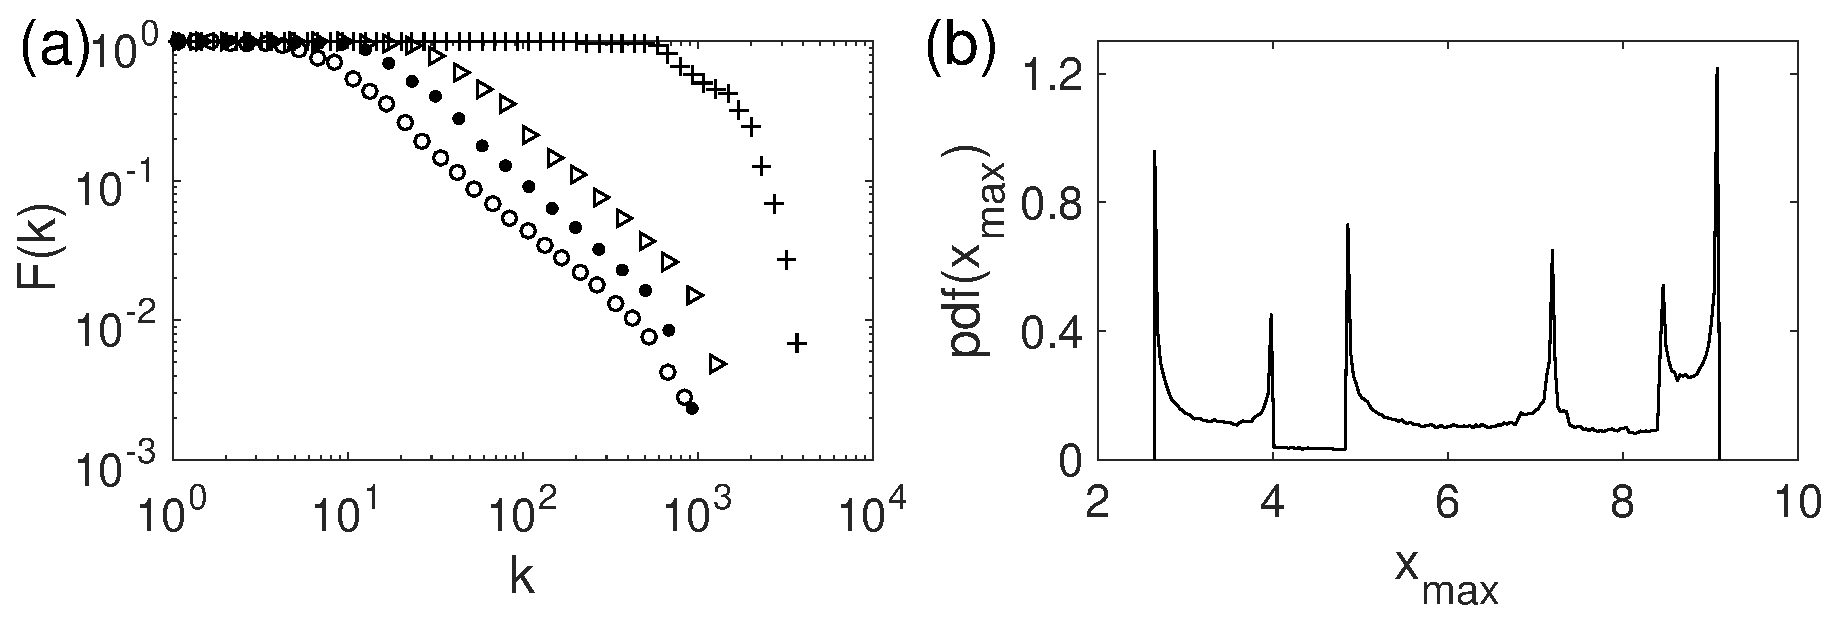
\includegraphics[width=\columnwidth]{Chapter03_RecurrenceNt/retmap_histP.eps}
	\caption{(a) Complementary cumulative distribution function $F(k)=\sum_{k'=k}^{\infty} p(k')$ for RNs obtained from the $x$-component of the first return map of the R\"ossler system (with $a=b=0.2$, $c=5.7$ in Eq.~\eqref{eq:roessler}) through the $y=0$ plane, using edge densities $\hat{\rho}_1 =0.02\%$ ($\circ$), $\hat{\rho}_2 =0.03\%$ ($\bullet$), $\hat{\rho}_3 =0.05\%$ ($\triangleright$), and $\hat{\rho}_4 =3\%$ (+). All curves have been obtained as mean values taken from $5$ independent realizations of the system with length $N=2\times 10^5$ and using the Euclidean norm. For $\hat{\rho}_1$ to $\hat{\rho}_3$, we find power-law behavior with a characteristic exponent of $\gamma=2.16\pm 0.03$, whereas no clear scaling region is found in the denser RN with edge density $\hat{\rho}_4$. (b) PDF of the $x$ values, where power-law shaped singularities are observed. Redrawn after \cite{Zou2012}.}
\label{fig:roessler_scaling}
\end{figure}

		Notably, it is not trivial to provide an exhaustive characterization of the conditions under which SF distributions can emerge for higher-dimensional systems. As a consequence, generally applicable necessary and sufficient conditions for the presence of power-laws in the degree distributions of RNs have not been established so far. Based on the degree distribution $p(k)$, some higher-order statistics have been proposed in \cite{Jocob2016} quantifying heterogeneity properties of the connectivity.

		We note that in general complex systems, the emergence of power-laws is often associated with a hierarchical organization related to certain fractal properties. In contrast, for RNs it has been shown that the presence of power-laws is not directly related to some (global) fractal structure of the system, but rather the local shape of its invariant density. Consequently, although there are examples of dynamical systems where the scaling exponent of the degree distribution coincides well with the associated fractal dimension, there is no such relationship in general. It will be a subject of future studies under which conditions regarding the structural organization of the attractor, fractal structure and power-law singularities are sufficiently closely related so that the RN's degree distribution allows quantifying the system's fractal properties.

       		 \subsubsection{Small-world effect}
		Since small-world networks are characterized by both, a high clustering coefficient and short average path length, it is clear that RNs cannot obey small-world effects \cite{Donner2015RPBook,Jacob2017,Jacob2018}: although they may exhibit a high degree of transitivity (typically depending on the specific system under study), for any \emph{fixed} value of $\varepsilon$, the average path lengths can only take specific values, which become independent of the network size $N$ in case of sufficiently large samples. On the one hand, for any chosen pair of vertices $i$ and $j$ at positions $\vec{x}_i$ and $\vec{x}_j$, the shortest path length is bounded from below as $\hat{d}_{ij}\geq \lceil\|\vec{x}_i-\vec{x}_j\|/\varepsilon\rceil$ (respectively, the geodesic distance on the attractor $S$ divided by the recurrence threshold $\varepsilon$). Specifically, each shortest path length will converge to a finite value for $N\to\infty$. On the other hand, due to the finite diameter of chaotic attractors, the average path length $\hat{\mathcal{L}}(\varepsilon)$ cannot exceed a maximum value of $\lceil\max_{i,j}\{\|\vec{x}_i-\vec{x}_j\|\}/\varepsilon\rceil$ independent of $N$. Hence, the average path length is bounded from above by a value independent of $N$, which is distinct from the common behavior of SW networks ($\hat{\mathcal{L}}\sim \log N$) \cite{Watts1998}. Moreover, as another immediate consequence of the latter considerations, we observe that $\hat{\mathcal{L}}\sim\varepsilon^{-1}$~\cite{Donner2010a}. This implies that by tuning $\varepsilon$, it is possible to achieve any desired average shortest path length $\hat{\mathcal{L}}$; this fact notably reduces the explanatory power of this global network characteristic. Adding sufficient amount of noise or increasing the threshold $\varepsilon$ comparable to the attractor size, SW properties may be numerically observed for RNs \cite{Jacob2016a,Jacob2017}.


		\subsubsection{Assortative vs. disassortative mixing}
		Unlike SW effects and SF degree distributions, there are hardly any available results regarding the mixing properties of RNs. In general, RNs often obey a tendency towards showing assortative mixing (i.e., vertices tend to link to other vertices with similar degree), which is reasonable in situations where the invariant density $p(\vec{x})$ is continuous or even differentiable, which is supported by recent numerical results \cite{Donges2011,Donner2010a}.

		\subsubsection{Path-based characteristics}\label{sec:apl}
		One main field of application of RQA as well as other quantitative approaches to characterizing the distribution of recurrences in phase space (e.g., recurrence time statistics) is identifying and quantifying different degrees of dynamical complexity among realizations of the same system under different conditions (e.g., different values of the control parameter(s)), or even within a single time series given the system is non-stationary \cite{marwan2007}. While the line-based characteristics of RQA are founded on heuristic considerations (e.g., the higher the predictability of the observed dynamics, the longer the diagonal line structures off the main diagonal should be), we have argued in Section~\ref{sec:analyticRNtheory} that RNs have an analytical foundation in RGGs. Notably, the corresponding characteristics are based on the same binary structure (the recurrence matrix) as the RQA measures. Hence, both concepts allow deriving a similar kind of information, with the important difference being that RQA quantifies dynamical properties, whereas RNs encode topological/geometric characteristics. However, since both aspects are ultimately linked in the case of chaotic attractors, this general observation suggests that RN analysis is in principle suitable for characterizing dynamical complexity in the same way as other established concepts. Therefore, one natural question arises: How do RN measures perform in this task, and which of the multiple possible network measures are particularly suited for this purpose?

		The latter questions have been the main motivation behind much of the early work on RNs focussing on numerical studies of various paradigmatic model systems for low-dimensional chaos~\cite{Donner2010Nolta,Donner2011,Donner2010b,Donner2010a,Marwan2009,Zou2010,Zou2012c}. These studies suggest that for characterizing dynamical complexity, global network characteristics are conceptually easier to use and could provide potentially more stable and distinctive results than certain statistics over local network properties such as the distributions of vertex degrees~\cite{Zou2012b} or local clustering coefficients~\cite{Zou2012c}. Among the set of possible global RN measures, two properties have been found particularly useful: network transitivity $\hat{\mathcal{T}}$ and average path length $\hat{\mathcal{L}}$.

		Regarding $\hat{\mathcal{L}}$, the discriminatory skills concerning different degrees of dynamical complexity can be understood by the fact that for time-continuous systems, chaotic systems can display different degrees of spatial filling of the ``populated'' hyper-volume in phase space, i.e., a high (fractal) dimension of a chaotic attractor close to the (integer) dimension gives rise to a more homogeneous filling than lower ones, which has a natural geometric consequence for the possible path lengths between pairs of sampled state vectors on the attractor. However, it needs to be noted that quantifying dynamical complexity by means of $\hat{\mathcal{L}}$ suffers from two important drawbacks:

		On the one hand, the measure is not normalized and depends crucially on the choice of $\varepsilon$. Hence, working in different methodological settings (e.g., using fixed recurrence thresholds $\varepsilon$ versus fixed recurrence rates $RR=\hat{\rho}$) can provide potentially ambiguous results, since numerical values of $\hat{\mathcal{L}}$ cannot necessarily be directly compared with each other.

		On the other hand, the system's dynamical complexity influences the qualitative behavior of $\hat{\mathcal{L}}$ , which further depends on whether the system is a discrete map or time-continuous. In the latter case, a periodic orbit would result in a higher $\hat{\mathcal{L}}$ than a chaotic one, since a chaotic attractor is a ``spatially extended'' object in phase space on which there are ``shortcuts'' between any two state vectors connecting points corresponding to different parts of the trajectory~\cite{Donner2010a}. In turn, for discrete maps, a periodic orbit contains only a finite set of $p$ mutually different state vectors, so that for sufficiently low $\varepsilon$ and large $N$, the RN is decomposed into $p$ disjoint, fully connected components. In such a situation with not just single isolated vertices, but a completely decomposed network, a reasonable redefinition of $\hat{\mathcal{L}}$ would be summing up only over pairs of mutually reachable vertices in Eq.~(\ref{eq:apl}). Consequently, we approach the minimum possible value of $\hat{\mathcal{L}}=1$~\cite{Marwan2009}, whereas chaotic orbits typically lead to larger $\hat{\mathcal{L}}$.

		According to the above observations, there is no fully developed theoretical understanding and description of the influence of attractor dimensionality on the resulting $\hat{\mathcal{L}}$ beyond the general considerations presented in Section~\ref{sec:analyticRNtheory}. Corresponding further investigations might be an interesting subject for future studies.

       		 \subsubsection{Dimension characteristics by clustering and transitivity} \label{sec:transitivity}
		As mentioned in Section~\ref{sec:scaling}, the scaling exponent of a possible power-law degree distribution has no direct relationship to the fractal dimension of the system \cite{Zou2012}. In turn, such a relationship naturally exists when studying the corresponding integrated measure (i.e., the edge density $\hat{\rho}(\varepsilon)$) in terms of its scaling properties as the recurrence threshold is systematically varied. The latter approach has been extensively discussed in the literature in connection with the estimation of dynamical invariants from RPs~\cite{Faure1998,thiel2004a} and gives rise to estimates of the correlation dimension $D_2$. Notably, one of the classical approaches to estimating $D_2$ from time series data, the Grassberger-Procaccia algorithm~\cite{Grassberger1983PLA,Grassberger1983PRL}, makes use of the correlation sum, which can be easily formulated as a special case in terms of the recurrence rate or RN edge density \cite{Faure1998}.

		The relatively high computational complexity of the latter approaches to estimating the correlation dimension from a RP stems from the fact that a sequence of RPs for different values of $\varepsilon$ needs to be studied for obtaining a proper scaling relationship. In turn, as shown in~\cite{Donner2011b}, network transitivity $\hat{\mathcal{T}}$ provides an alternative approach to defining and estimating a different notion of fractal dimension. For this purpose, note that for a classical RGG embedded in some integer-dimensional metric space, the expected $\hat{\mathcal{T}}$ (which is numerically estimated as the ensemble mean over sufficiently many realizations of the stochastic generation of the RGG) is an analytical function of the dimension $m$, which decays (exactly when using the maximum norm, otherwise approximately) exponentially with $m$~\cite{Dall2002}. This analytical relationship can be generalized to attractor manifolds with non-integer fractal dimensions, which can in turn be estimated from the RN transitivity by inverting this function.

		\paragraph{Transitivity dimensions}
		For the general case, the idea formulated above leads to a pair of quantities referred to as upper and lower transitivity dimensions \cite{Donner2011b},
\begin{eqnarray}
D_{\mathcal{T}}^u &=& \limsup_{\varepsilon} \frac{\log(\mathcal{T}(\varepsilon))}{\log(3/4)}, \label{eq:dtu} \\
D_{\mathcal{T}}^l &=& \liminf_{\varepsilon} \frac{\log(\mathcal{T}(\varepsilon))}{\log(3/4)}, \label{eq:dtl}
\end{eqnarray}
\noindent
where the two definitions originate from the fact that certain systems (in particular, chaotic maps whose attractors form Cantor sets in at least one direction in phase space~\cite{Donner2011b}) can exhibit an oscillatory behavior between some upper and lower accumulation point of $\mathcal{T}(\varepsilon)$ as the recurrence threshold $\varepsilon$ is varied (Fig.~\ref{fig:roessler_transitivity}(a)). For systems without such fragmented structure, the upper and lower transitivity dimensions practically coincide, which allows estimating them from the sample RN transitivity with reasonable accuracy using only a single network instance with one suitably chosen value of $\varepsilon$. A detailed analytical investigation of the qualitatively different behavior of the RN transitivity for chaotic attractors with continuous and fragmented invariant densities in dependence on $\varepsilon$ will be subject of future work. Note that in the above definition, we do not explicitly consider a scaling behavior for $\varepsilon\to 0$, since the definition does not explicitly contain $\varepsilon$ (as it is the case for other classical notions of fractal dimensions), but makes use of normalized characteristics with a probabilistic interpretation (cf. Section~\ref{sec:analyticRNtheory}). In this spirit, the fraction on the right-hand side of the Eqs.~\eqref{eq:dtu} and \eqref{eq:dtl} is a well-defined object for each value of $\varepsilon$ (i.e., the specific scale under which the system is viewed) individually.
\begin{figure}
\centering
\includegraphics[width=\columnwidth]{Chapter03_RecurrenceNt/transitivity3_dim_convergence.eps}
\caption{(a) Transitivity dimensions $\hat{D}_{\mathcal{T}}$ of the H\'enon map (Eq.~\ref{eq:henon} for one realization with initial condition $(x, y) = (0, 0)$, the first 1000 iterations have been removed from the trajectory to avoid transient behavior) for different $N$. Dashed horizontal lines indicate numerical estimates $\hat{D}_{\mathcal{T}}^{u, l}$ (Eqs. (\ref{eq:dtu}, \ref{eq:dtl})). (b) Same for the R\"ossler system (Eq.~\ref{eq:roessler}) with different lengths $N$ (sampling time $\Delta t=0.05$, first part of the trajectory removed to avoid possible transient dynamics). Note the different scale on the $x$ axis. Modified from \cite{Donner2011b}. } \label{fig:roessler_transitivity}
\end{figure}
Figure~\ref{fig:roessler_transitivity} shows the behavior of the scale-dependent transitivity dimension estimate $\hat{D}_{\mathcal{T}}(\varepsilon)=\log(\hat{\mathcal{T}}(\varepsilon))/\log(3/4)$ for the H\'enon map (Eq.~\ref{eq:henon}) and the R\"ossler system (Eq.~\ref{eq:roessler}) for three different RN sizes. We note that very long realizations are typically required to numerically capture the local features of the chaotic attractor of the H\'enon map with reasonable confidence as shown in Fig.~\ref{fig:roessler_transitivity}(a). The larger $N$, the better the estimated values of this measure obtained for fixed $\varepsilon$ approach stationary values corresponding to the upper and lower transitivity dimensions. In contrast, for too small $N$, we observe significant deviations from the asymptotically estimated values, which becomes particularly important for $\varepsilon \to 0$.

		In the case of the R\"ossler system, we obtain similar results shown in Fig. \ref{fig:roessler_transitivity}(b).  We clearly recognize that $\hat{D}_{\mathcal{T}}(\varepsilon)$ assumes approximately stable (i.e., $N$- and $\varepsilon$-independent) values if the recurrence threshold is chosen sufficiently large. In general, there exist two limits that need to be taken into account: For too large recurrence rates, the RN characteristics lose their discriminatory skills, since too many edges are present masking subtle small-scale properties of the attractor \cite{Donner2011b,Donner2010b}. In turn, if $\varepsilon$ is too low (e.g., if $\hat{\rho}$ is below the RN's percolation threshold) \cite{Donges2012}, the network decomposes into mutually disjoint components, and the resulting network characteristics can become ambiguous. In the considered example of the R\"ossler system, this decomposition is mainly caused by the rare excursions of some cycles towards larger $z$ values, which give rise to a poorly populated region (low $p(\vec{x})$) of the attractor. In order to properly cover this part of the attractor for a given $\varepsilon$, many samples (i.e., a large network size $N$) are necessary. Otherwise, the edge density $\hat{\rho}$ starts saturating as $\varepsilon$ gets smaller (at least in the regime where most vertices close to the $z=0$ plane are still connected, cf.\, Fig.~\ref{fig:roessler_transitivity}(b)), and the transitivity dimension estimates strongly deviate from their expected values.

		Notably, the analytical relationship in Eqs.~(\ref{eq:dtu}), (\ref{eq:dtl}) between the effective (geometric) dimension of chaotic attractors and RN transitivity provides the theoretical justification and foundation for applying $\hat{\mathcal{T}}$ as a characteristic discriminating between high and low dynamical complexity of chaotic attractors. Unlike for $\hat{\mathcal{L}}$, the transitivity shows qualitatively the same behavior for discrete and time-continuous systems and is normalized, so that its values can be directly used as a quantitative measure of dynamical complexity associated with the effective geometric dimensionality and, hence, structural complexity of the attractor in phase space.


		\paragraph{Local clustering dimensions}\label{sec:transitivitylocal}
		With the same rationale as for the global network transitivity, we can make use of the local clustering properties of RNs for defining local measures of attractor dimensionality, referred to as upper and lower clustering dimensions~\cite{Donner2011b}:
\begin{eqnarray}
D_{\mathcal{C}}^u(\vec{x}) &=& \limsup_{\varepsilon} \frac{\log(\mathcal{C}(\vec{x};\varepsilon))}{\log(3/4)}, \\
D_{\mathcal{C}}^l(\vec{x}) &=& \liminf_{\varepsilon} \frac{\log(\mathcal{C}(\vec{x};\varepsilon))}{\log(3/4)}.
\end{eqnarray}
\noindent
Following the same argument as for the (global) transitivity dimensions, we do not need to consider the limit $\varepsilon\to 0$ here.

		With similar considerations regarding the possible existence of two distinct accumulation points of $\mathcal{C}(\vec{x})$ as $\varepsilon$ varies, we may utilize this framework for characterizing the point-wise dimension of chaotic attractors in a unique way without making explicit use of scaling characteristics as in the common point-wise dimensions~\cite{Donner2011b}. However, we need to keep in mind that the considered concept of (geometric) dimensionality is largely affected by the profile of the invariant density, e.g., the existence of sharp attractor boundaries or supertrack functions~\cite{Donner2010Nolta,Donner2011b,Donner2010a}. For example, if the attractor has distinct tips (e.g., in the case of the H\'enon system~\cite{Donner2011b,Donner2010a}), the geometric dimension at these points is effectively reduced to zero, which is reflected by $\hat{\mathcal{C}}_i=1$ for state vectors $\vec{x}_i$ sufficiently close to the tips. A similar behavior can be observed for the logistic map at the attractor boundaries and the supertrack functions~\cite{Donner2010Nolta,Donner2011b,Donner2010a}.

		The latter observations point to a prospective application of the local clustering properties of RNs. In case of chaotic attractors of time-continuous dynamical systems, it is known that an infinite number of unstable periodic orbits (UPOs) provide the skeleton of the chaotic dynamics and they are densely embedded in the attractor. The localization of such UPOs is, however, known to be a challenging task. Since UPOs are relatively weakly repulsive (from a practical perspective, those UPOs with low periods are typically least unstable), a trajectory getting close to the vicinity of an UPO will stay close to this orbit for some finite amount of time~\cite{Lathrop1989}. As a result, the dynamics close to UPOs is quasi one-dimensional, and state vectors sampled from the trajectories approximate some lower-dimensional (in the limiting case one-dimensional) subset of the attractor manifold. In such a case, the above theoretical considerations suggest that the local clustering coefficient $\hat{\mathcal{C}}_i$ of vertices $i$ close to low-periodic UPOs should be higher than the values typical for other parts of the chaotic attractor. This conceptual idea is supported by numerical results from~\cite{Donner2010b,Donner2010a} (cf.\, also the band structures with increased $\hat{\mathcal{C}}_i$ in Fig.~\ref{fig:local}(b)), but has not yet been systematically applied to the problem of UPO localization. Notably, the detection limit of UPOs should be ultimately determined by the recurrence threshold $\varepsilon$ in conjunction with the RN size $N$. Specifically, for every finite $\varepsilon>0$, there are infinitely many UPOs intersecting with the $\varepsilon$-neighborhood of some point $\vec{x}_i$ in phase space, whereas we will (for a finite sample of state vectors) only resolve the signatures of the least unstable orbits.


	\subsection{Practical considerations} \label{subsec:practicalRN}

The impact of several algorithmic parameters such as recurrence threshold $\varepsilon$, embedding parameters, sampling rate, or even the selection of variables in multi-dimensional systems has been extensively discussed in previous works~\cite{Donner2010b,Strozzi2009}, focusing mostly on deterministic systems, but also addressing stochastic ones recently. In the following, we will summarize the main findings that should guide corresponding methodological choices in practical applications of RN analysis.


		\subsubsection{Choice of recurrence rate or threshold} \label{subsub:epsilon}
		The most crucial algorithmic parameter of recurrence-based time series analysis is the recurrence threshold $\varepsilon$, which has been discussed extensively in the literature \cite{marwan2007,Donner2010b,Donges2012,Jacob2017}. The empirical choice of $\varepsilon$ often depends on time series embedded in phase space. Too small $\varepsilon$ causes very sparsely connected RNs with many isolated components; too large $\varepsilon$ results in an almost completely connected network. Several invariants of a dynamical system, e.g., the second-order R\'enyi entropy $K_2$  can be estimated by taking its recurrence properties for $\varepsilon \to 0$ \cite{Grassberger1983PLA,Grassberger1983PRL}, which suggests that for a feasible analysis of RNs, a low $\varepsilon$ is preferable as well. This is supported by the analogy to other types of complex networks based on spatially extended systems, where attention is usually restricted to the strongest links between individual vertices, i.e., observations from different spatial coordinates for retrieving meaningful information about relevant aspects of the systems' dynamics. In contrast, a high edge density, does not yield feasible information about the actually relevant structures, because these are hidden in a large set of mainly less important edges \cite{Donner2010b,Donges2012,Jacob2017}.

		As a consequence, only those states should be connected in a RN that are closely neighbored in phase space, leading to rather sparse networks. Following a corresponding rule of thumb confirmed for recurrence quantification analysis \cite{schinkel2008}, one common choice of $\varepsilon$ would be corresponding to an edge density $\rho \lesssim 0.05$ \cite{Marwan2009,Donner2010a}, which yields neighborhoods covering appropriately small regions of phase space. Note that since many topological features of recurrence networks are closely related to the local phase space properties of the underlying attractor~\cite{Donner2010a}, the corresponding information is best preserved for such low $\varepsilon$ unless the presence of noise requires higher $\varepsilon$ \cite{schinkel2008}.

		The heuristic criterion selecting $\varepsilon$ as the (supposedly unique) turning point of the plot of $\rho$ versus $\varepsilon$ \cite{Gao2009} is not generally applicable (as discussed in \cite{Donner2010b}). In particular, this heuristic criterion cannot attribute certain network features to specific \textit{small-scale} attractor properties in phase space \cite{Donner2010b}. Moreover, besides our general considerations supporting low $\varepsilon$, application of the turning point criterion can lead to serious pitfalls. We have to emphasize that various typical examples for both discrete and continuous dynamical systems are characterized by \textit{several} turning points. Depending on the particular types of signals from real measurements from civil engineering structures, a surrogate-assisted method for choosing an optimal threshold by searching for a turning point of a properly defined quality loss function might be a good solution \cite{Yang2015a}.

		For meaningfully estimating path-based and other higher-order structural properties of recurrence networks it is important that the recurrence network possesses a giant component and, hence, nearly all nodes are reachable from nearly all other nodes. At the same time, $\varepsilon$ should be as small as possible so that geometrical fine structure of the underlying attractor is still reflected in the recurrence network. Donges et al. propose to make use of this insight and suggest to set the recurrence threshold just above the percolation threshold $\varepsilon_c$ of the random geometric graph corresponding to the invariant density underlying the dynamical system under study \cite{Donges2012}. This approach allows to connect the problem of choice of recurrence threshold to insights from the theory of random geometric graphs \cite{Dall2002,penrose2003random,herrmann2003connectivity} and, more generally, spatial networks \cite{Gastner2006e,Barthelemy2011,Wiedermann2016} on the percolation threshold $\varepsilon_c$ or the more frequently critical mean degree $z_c(\varepsilon_c)$ in random geometric graphs. In this way, the method allows to make use of analytical results on $z_c$ that have been obtained for various geometries and invariant densities \cite{Dall2002}. These show that the percolation threshold $z_c=1$ of Erd\H"os-R\'enyi graphs is not a tight lower bound for random geometric graphs, i.e. also not in the case of RNs, but that the true critical mean degree tends to be larger due to spatial clustering effects. For example, \textit{Dall and Christensen}\cite{Dall2002} empirically find a scaling law
		\begin{equation}
		z_c(d) = z_c(\infty) + A d^{-\gamma}
		\end{equation}
		for the $d$-dimensional box $S=[0,1]^d$ with uniform probability density $p$, where $z_c(\infty) = 1$, $\gamma = 1.74$, and $A = 11.78$. Alternatively, $\varepsilon_c$ can be obtained from the available data point cloud by numerical methods, e.g., efficiently by $k$-d tree algorithms.

        		One of the problems preventing a uniform choice of $\varepsilon$ across different time series is that the size of the attractor after embedding is arbitrary. To overcome this, Jacob {\textit{et~al.}} \cite{Jacob2016b,Jacob2016a} proposed first to normalize the time series into a unit interval so that the size of the attractor gets rescaled into the unit cube $[0, 1]^m$ where $m$ is embedding dimension. Then, their choice of $\varepsilon$ has been based on empirical results from numerical computations such that the following two criteria are fulfilled \cite{Jacob2016b}: (a) the resulting RN has to remain mostly as ``one single cluster" (see also \cite{Donges2012}) and (b) the measures derived from the RN should uniquely represent the underlying attractor. The first condition fixes the lower bound for $\varepsilon$ which ensures that the network becomes fully connected. The second one fixes the upper bound. Furthermore, Jacob \emph{et~al.} showed that the above two conditions together provide an identical optimum $\varepsilon$ range for time series from all chaotic attractors. However, recent findings point to the fact that this range may still depend on the specific system under study and, more importantly, on the embedding dimension $m$ controlling the distribution of pairwise distances between state vectors in phase space, which should guide the corresponding threshold selection \cite{Kraemer2018}. Moreover, it should be noted that the above choice of the critical range of $\varepsilon$ is, in fact, conceptually related to the selection of a scaling region in the conventional nonlinear time-series analysis for computing dynamical invariants like the correlation dimension $D_2$ \cite{Grassberger1983PLA}, thereby relieving the potential advantage of RN properties providing scale-local characteristics related to such dynamical invariants \cite{Donner2011b}.

		The above strategies for choosing $\varepsilon$ based on normalizing the underlying time series or fixing the recurrence density help us to overcome the problem of sliding-window-based analyses of systems with varying amplitude fluctuations (as coming from different dynamical regimes or non-stationarities). However, in real-world applications, time series are usually not always smooth. When considering time series by studying their RN representations, extreme points (very high rises or falls in the fluctuations) in the time series could break the connected components in the network since the distance between an extreme point and other points would be larger than the threshold value \cite{Eroglu2014}. These unconnected components would cause problems for some complex network measures, since some of them need a connected network to be computed for the entire network. For example, even if we have just one node that is not connected to the network, the average path length will always be infinite for the entire network unless employing the artificial definition of $l_{ij}=N$ for vertices in disconnected components. In such a situation, the normalization method of Jacob \emph{et~al.} \cite{Jacob2016b,Jacob2016a} would result in non-optimal recurrence thresholds biasing the recurrence analysis. An even more important motivation for avoiding isolated components in a RN is that the RN provides a large amount of information about the dynamics of the underlying system, although it contains only binary information. To find a sufficiently small threshold $\varepsilon$ that fulfills the desired condition of connected neighborhoods, Eroglu {\textit{et al.}} proposed to use the connectivity properties of the network. In particular, here the value for $\varepsilon$ is chosen in such a way that it is the smallest one for the RN to be connected. The connectivity of a RN is measured by the second-smallest eigenvalue $\lambda_2$ of the Laplacian matrix associated to the RN's adjacency matrix \cite{Eroglu2014}. Note that this criterion for choosing $\varepsilon$ in an adaptive way shares the same idea as \cite{Jacob2016b,Lin2016}. In the special case where the phase space consists of several disjoint partitions, the method guaranteeing the connectivity might not be feasible, for instance, the support of the invariant density is not continuous when the control parameter is in the periodic or even chaotic regimes before the band merging crisis of the logistic map. Another example for such a behavior is the standard map, where there exist several spatially disjoint components of periodic dynamics in phase space \cite{Donner2010b,Zou2016d}).

		 Note that modular regions of RNs may correspond to a trajectory bundle, which can be associated with the existence of metastable states. Small variations of $\varepsilon$ may lead to very different modular structure in the associated RN, which poses a big challenge for identifying metastable states in real-world time series. Choosing an inadequate recurrence threshold can hide important geometric information related to the organization of a system in its phase space. In \cite{Vega2016}, it was suggested that an adequate recurrence threshold should lie in a range of values producing RNs with similar modular structures. This means that there is a range of recurrence thresholds for which the associated RNs describe reconstructed state space objects with equivalent topology. However, this region of values depends on the distribution of the particular time series data, which might not be uniform. Therefore, they define a filtration procedure to self-adaptively set an adequate $\varepsilon$ from RNs that are associated to a set of recurrence thresholds. The adequate $\varepsilon$ belongs to the subset of values in the filtration for which the modular structures of their associated RNs are the least dissimilar. Furthermore, in searching for metastable states \cite{Vega2016}, the authors suggested to compute modular similarity measures like the adjusted rank index, which may further help to identify an adequate recurrence threshold $\varepsilon$.
Finally, a more recent alternative approach to the threshold selection problem in RNs has been suggested by Wiedermann \emph{et~al.} \cite{Wiedermann2017} in terms of analyzing the statistical complexity of the resulting RNs based upon the Jensen-Shannon divergence between their mean random-walker entropy $\mathcal{S}^{RW}=\sum_{i} \log k_i /N\log(N-1)$ and that of ER random graphs. Specifically, they argued that the threshold could be chosen such that the resulting RN structure becomes most informative, which could be measured in terms of this specific complexity measure. However, it might be questioned if the most complex network structure also corresponds to the most informative one, e.g., when considering the selection of the corresponding edge density as a statistical model selection problem with the network's statistical complexity as the target function to be optimized and the number of links as an analog to the number of degrees of freedom that should be used for penalizing the target function. Additional theoretical work will be necessary to further address this problem.


		\subsubsection{Dependence on embedding parameters} \label{subsubsec:embedding}
Two other important algorithmic parameters of the RN approach are the parameters of time-delay embedding, i.e., embedding dimension $m$ and delay $\tau$. Note that alternative approaches of phase space reconstruction are possible, particularly so-called derivative embedding, which are however often harder to use and would just replace the embedding delay by other parameters possibly involved in more complex algorithms \cite{Lekscha2018}. For this reason, we will not further discuss these alternative approaches here.

		As mentioned in Section \ref{sec:attractorReconstruct}, our discussion so far has assumed that proper embeddings are available for the given time series. For instance, embedding dimension $m$ and delay $\tau$ could have been chosen properly by means of the FNN and ACF method, respectively, which commonly works well for data from deterministic dynamical systems. In turn, proper embeddings do not exist for non-stationary processes though they are more ubiquitous in real time series analysis, for instance, fractional Brownian motions (fBm) and related processes arising from an integration of stationary processes (e.g., fractional L\'evy motion, (F)ARIMA models, etc.). More specifically, we have to keep in mind that some severe conceptual problems may appear when applying them to non-stationary processes: First, finite estimates of $D_F$ are spurious due to the finite amount of data used. The latter result is reasonable since an infinite amount of data (i.e., the innovations at each time step) are necessary to fully describe the evolution of a stochastic process. Thus, from a conceptual perspective, the embedding dimension should be chosen infinitely large. In turn, finite $m$ will necessarily cause spurious results, since the full complexity of the system's (discrete) trajectory is not captured.

		On the other hand, the embedding delay $\tau$ is not considered in the mathematical embedding theorems for deterministic dynamical systems. Embeddings with the same embedding dimension $m$ but different $\tau$ are topologically equivalent in the mathematical sense~\cite{kantz1997}, but in reality a good choice of $\tau$ facilitates further analysis. If $\tau$ is small compared to the relevant internal time-scales of the system, successive elements of the delay vectors are strongly correlated. This leads to the practical requirement that the embedding delay should cover a much longer time interval than the largest characteristic time-scale that is relevant for the dynamics of the system. However, in fBm arbitrarily long time-scales are relevant due to the self-similar nature of the process \cite{Zou2015}. This makes finding a feasible value of $\tau$ a challenging (and, regarding formal optimality criteria, even theoretically impossible) task.

		We emphasize that in the case of non-stationary fBm, the fundamental concepts of phase space reconstruction and low-dimensional dynamics do not apply (not even approximately) anymore. Therefore, the corresponding RN results as have been presented in \cite{Liu2014} hold only for the particular choices of the algorithmic parameters (for instance, length of time series, embeddings etc), showing limited physical interpretations. In \cite{Zou2015}, it has been demonstrated that RN analysis can indeed provide meaningful results for stationary stochastic processes, given a proper selection of its intrinsic methodological parameters, whereas it is prone to fail to uniquely retrieve RN properties for intrinsically non-stationary stochastic processes like fBm. In cases of non-stationarity, a proper transformation is required to remove the particular type of non-stationarity from the data. This can be achieved by additive detrending, phase adjustment (de-seasonalization), difference filtering (incrementation) or other techniques, with the one mentioned last being the proper tool for the particular case of fBm transforming the original process into stationary fractional Gaussian noise (fGn). Further numerical results on the RN analysis for fGn will be presented in Section \ref{subsubsec:nonstation}.


		 \subsubsection{$\varepsilon$-dependence of RN properties}
		 In order to evaluate the robustness of the topological properties of RNs, their dependence on the free parameter of the method, $\varepsilon$, has to be explicitly considered. In particular, we show in Fig.~\ref{avg_path_all} the effects of $\varepsilon$ on network measures $\hat{\mathcal{L}}$ and $\hat{\mathcal{C}}$. The scale dependence of $\hat{\mathcal{T}}$ has been briefly reviewed in Section \ref{sec:transitivity} and further results of $\hat{\mathcal{T}}$ and $\hat{\mathcal{R}}$ can be found in \cite{Donner2010a,Donner2011b}. In the following, we briefly summarize the main findings for the three model systems H\'enon map (Eqs.~\ref{eq:henon}), R\"ossler (Eqs.~\ref{eq:roessler}), and Lorenz system (Eqs.~\ref{eqlorenz}).
		 \begin{figure}
  		\centering
  			\includegraphics[width=\columnwidth]{Chapter03_RecurrenceNt/avg_henon_ros_lrz_eps.eps} \\
  			\includegraphics[width=\columnwidth]{Chapter03_RecurrenceNt/ccavg_Henon_Ros_Lrz.eps}  \\
		\caption{\small Dependence of the average path length $\mathcal{L}$ (a-c) and the global clustering coefficient $\mathcal{C}$ (d-f) for the H\'enon map (Eqs.~\ref{eq:henon}), R\"ossler (Eqs.~\ref{eq:roessler}), and Lorenz system (Eqs.~\ref{eqlorenz}) (from left to right). Dashed lines in the plots on $\hat{\mathcal{L}}(\varepsilon)$ indicate the approximate presence of the theoretically expected $1/\varepsilon$ dependence of $\hat{\mathcal{L}}$. Reproduced from \cite{Donner2011}. }  \label{avg_path_all}
		\end{figure}

		 As we already discussed associated with Eq.~\eqref{avgL_eq} in Section~\ref{subsubsec:RNmeasureG}, there is an inverse relationship between $\hat{\mathcal{L}}$ and the threshold $\varepsilon$, which has been numerically confirmed in Fig.~\ref{avg_path_all}(a, b, c). However, for the global clustering coefficient $\hat{\mathcal{C}}$, the dependence on $\varepsilon$ is more complicated and depends on the specific properties of the considered system (Fig.~\ref{avg_path_all}(d, e, f)). In particular, while for too small $\varepsilon$, problems may occur, since the RNs will generally decompose into different disconnected clusters for a length $N$ of the considered time series, for intermediate threshold values, an approximately linear increase of $\hat{\mathcal{C}}$ with $\varepsilon$ seems to be a common feature of all three examples.

		\subsubsection{Stability and robustness against noise}
        		The results presented in Section~\ref{sec:transitivity} together with the numerical findings for model systems that will be presented in Section~\ref{sec:numex} show that RN approaches are able to clearly distinguish between periodic and chaotic dynamics under noise-free condition. However, in experimental time series, one is always confronted with measurement errors. Hence, it is necessary to analyze the influence of noise on the constructed RNs. In the framework of recurrence plots, choosing a larger $\varepsilon$ has been suggested to overcome the effect of additive noise \cite{thiel2002}, e.g., using a threshold $\epsilon$ that is at least 5 times larger than the standard deviation $\sigma$ of the observational Gaussian noise can yield reliable statistics. This criterion is based on an analytical computation of the probability of a recurrence point in the RP to be correctly recognized in the presence of observational noise. We suggest to use this criterion if weak observational noise is present as it has been found that the choice $\epsilon \sim 5\sigma$ is optimal for a wide class of processes \cite{thiel2002}.

		It is interesting to visualize noise effects on the reconstructed RNs, which have been presented in \cite{Jacob2016a}. In this work, the authors found numerically that RNs retain much of the information regarding the shapes of the attractor even with moderate addition of both, white and colored noise. Their numerical results suggest that the topology of RNs may completely change if the noise contamination level is above 50\% of signal-to-noise ratio. Furthermore, it has been shown in \cite{Subramaniyam2014} that the influence of noise on the clustering coefficient $\mathcal{C}$ can be minimized by an appropriate choice of $\rho(\varepsilon)$ (e.g., by setting $\rho(\varepsilon) > 0.02$), while the influence on the average path length $\mathcal{L}$ is independent of $\rho(\varepsilon)$. However, for noise levels greater than 40\% in case of $\mathcal{C}$ and 20\% in case of $\mathcal{L}$, the RN measures fail in distinguishing between noisy periodic dynamics and noisy chaotic dynamics. As the noise level reaches 50\% or more, the structural characteristics of RNs present a smooth transition to those of random geometric graphs \cite{Jacob2017}. In particular, Jacob {\textit {et~al.}} have numerically shown that these transitions hold for degree distributions, clustering coefficients and shortest path length \cite{Jacob2017}. The cross-over behavior of RNs towards random graphs has also been observed if $\varepsilon$ is increased towards the system size \cite{Jacob2017}. For large $\varepsilon$, the degree distributions tend to become Poissonian and both, clustering coefficient and shortest path length tend to be $1$, which are characteristics for random networks with very high edge density.

		By no means one can avoid noise effects when applying RN measures to discriminate different dynamical properties from experimental time series. In order to test the efficiency of RN measures as discriminating statistics, hypothesis testing using surrogate technique has been recently proposed \cite{Jacob2018}. For instance, a hypothesis that the data are derived from a linear stochastic process has been employed in \cite{Jacob2018}. The numerical results show that the clustering coefficient $\mathcal{C}$ is not a good discriminating measure if the data involves colored noise whereas the shortest path length $\mathcal{L}$ is effective in the presence of both white and colored noise. We have to emphasize that the specific choice of the hypothesis is fundamental to the interpretation of such results.

		More generally, the consideration of uncertainties plays a crucial role for experimental time series. There are various sources of uncertainties, including measurement errors, noise, irregularly distributed sampling times, etc. The importance of considering the type and magnitude of the uncertainties of an observable in time series analysis cannot be stressed enough. In \cite{Goswami2018}, Goswami {\textit{et~al.}} introduced a framework that merges the analysis of the measurements with that of their uncertainties, including uncertainties in the timing of observations, and shifts the focus from knowing the value of an observable at a given time to knowing how likely it is that the observable had a specific value at that time. In this case, since we consider time series with uncertainties, it is not possible to give a precise answer to the question whether time points $i$ and $j$ recurred, in the sense that we cannot answer this question with a $1$ or $0$ as in a traditional recurrence analysis. We estimate instead the probability that the observations at times $i$ and $j$ are contained in their respective $\varepsilon$-neighborhood. A further point of difference with traditional recurrence analysis is that, till date, there does not exist any meaningful way to embed a time series of probability densities, and one thus estimates the recurrence probabilities in the following without embedding. This novel framework of recurrence probabilities helps to track abrupt transitions in real time series with much improved statistical significance \cite{Goswami2018}. We emphasize that uncertainties bring a huge challenge to complex network approaches to nonlinear time series analysis in general. We will continue the corresponding discussions when reviewing the visibility graph methods in Section~\ref{secsec:VGpractical}.

	\subsection{Numerical examples}\label{sec:numex}
	%Here we show several successful yet specific applications of RN approaches by numerical models.
		RN approaches have been widely used for disentangling different dynamical regimes in different times of both, time-discrete and time-continuous dissipative systems \cite{Marwan2009,Donner2010a,Donner2010b,Donner2011,Donner2011b,Zou2010}. Specifically, as discussed above, discriminating qualitatively different types of dynamics can be achieved in terms of measures of complexity, dynamical invariants, or even structural characteristics of the underlying attractor's geometry in phase space. In the context of RN, local vertex-based network characteristics of time series can be visualized in the corresponding phase space as shown in Fig.~\ref{fig:local} \cite{Donner2010a}. For instance, phase spaces of discrete logistic and H\'enon maps, as well as the chaotic R\"ossler and Lorenz system have been color coded by vertex degrees $\hat{k}_i$, local clustering coefficient $\hat{\mathcal{C}}_i$ and betweenness $\hat{b}_i$, respectively \cite{Donner2010a,Donner2010Nolta,Donner2011,Donner2011b}. Furthermore, global network measures like transitivity $\hat{\mathcal{T}}$ or average path length $\hat{\mathcal{L}}$ have been applied to identify dynamical transitions in the logistic map when the control parameter is changed \cite{Marwan2009}. In addition to such stationary settings, the effect of drifting parameters on such characteristics has also been studied for classical model systems in terms of some sliding window analysis \cite{Donges2011}.

In the following, we will briefly review some ``non-classical'' numerical examples illustrating to which extent the aforementioned studies can be generalized to the contexts of higher-dimensional parameter spaces, Hamiltonian or even stochastic dynamics.


		\subsubsection{Parameter space in the R\"ossler system}
		In order to further illustrate the performance of RN transitivity $\hat{\mathcal{T}}$ and average path length $\hat{\mathcal{L}}$ as tracers for qualitative changes in the dynamics of complex systems, we briefly recall results originally obtained by the authors of \cite{Zou2010}. In the latter work, the RN properties have been successfully used to discriminate between periodic and chaotic solutions in a two-dimensional subspace of the complete three-dimensional parameter space $(a,b,c)$ of the R\"ossler system. As Fig.~\ref{fig:roessler_shrimp} reveals, there are sequences of transitions between periodic and chaotic solutions. Specifically, we clearly see that the periodic windows are characterized by higher values of $\hat{\mathcal{T}}$ and $\hat{\mathcal{L}}$ than the chaotic solutions, which is in agreement with the general considerations in Sections~\ref{sec:apl} and \ref{sec:transitivity}. Specifically, for the periodic windows, we find $\hat{\mathcal{T}}$ close to $0.75$, the theoretical value for periodic dynamics (i.e., a system with an effective dimension of $1$).
		\begin{figure}
		\centering
			\includegraphics[width=\columnwidth]{Chapter03_RecurrenceNt/ros_shrimp_eBook.eps}
		\caption{RN transitivity $\hat{\mathcal{T}}$ (A) and average path length $\hat{\mathcal{L}}$ (B) for a two-dimensional intersection ($a=b$) of the three-dimensional parameter space of the R\"ossler system (Eq.~\ref{eq:roessler}), displaying ``shrimp'' structures (i.e., self-similar periodic windows with complex shape). For details, see~\cite{Zou2010}.}
\label{fig:roessler_shrimp}
\end{figure}

		In a similar way, we may use the RN framework for capturing the signatures of qualitative changes in the attractor's shape and invariant density as a single control parameter is varied systematically. In a previous study using the R\"ossler system, the RN properties across the transition from the classical phase-coherent R\"ossler attractor to the non-coherent funnel regime have been investigated in \cite{Zou2012c}. Our results indicate that phase coherence -- in a similar spirit as fractal dimension -- can be characterized from a geometric rather than a dynamics viewpoint. However, as of today there is no single RN-based index for phase coherence that has been explicitly derived from theoretical considerations.


\subsubsection{Hamiltonian dynamics}

		In \cite{Zou2016d}, the validity of the RN approach for achieving the same goals in low-dimensional Hamiltonian systems has been demonstrated. Using the standard map as a paradigmatic example, RN analysis was applied to distinguish between regular and chaotic orbits co-existing in the same phase space. Specifically, it was shown (see below) that sticky orbits of the standard map (Eqs.~\ref{std_map_book}) can have a distinct geometric organization that can be detected reliably by RN analysis of relatively short time series (say, $N=1,000$ or $5,000$ points). Note that this model is probably the best-studied chaotic Hamiltonian map and can be interpreted as a Poincar\'e section of a periodically kicked rotor \cite{Lichtenberg_Lieberman_regular,Meiss_rmp_1992}.

		As in other Hamiltonian systems, the phase space of the standard map presents a complicated mixture of domains of chaotic trajectories coexisting with domains of regular ones. The regular component consists of both periodic and quasi-periodic trajectories, while the irregular one contains one or more chaotic orbits. A typical chaotic trajectory needs a long time to fill its corresponding domain in phase space. Due to the existence of periodic islands, once a chaotic orbit gets close to such an island, it can stay close to it and be almost regular in its motion for a rather long time. After this transient period it escapes again to the large chaotic sea. Such a long-term confinement of the trajectory close to the regular domain is commonly referred to as stickiness \cite{Karney_physicaD_1983,Meiss_rmp_1992}, which has been accepted as a fundamental property of many Hamiltonian systems.

The corresponding results for the three global RN measures $\hat{\mathcal{T}}, \hat{\mathcal{C}}$ and $\hat{\mathcal{L}}$ are shown in Figs.~\ref{fig:sm_rec_rr}. Here, we choose 200 initial conditions distributed randomly within the domain of definition of the standard map, $(x,y) \in [0, 1] \times [0, 1]$, and use the canonical parameter value of $\kappa = 1.4$ in Eqs.~\eqref{std_map_book}. All trajectories are computed for $5000$ time steps. Since we were aiming for a quantitative comparability of RN characteristics (which can depend on $RR$), we adaptively choose $\varepsilon$ such that the $RR$ has the same fixed value \cite{Zou2016d}. We observe that the overall structure of the phase space with its intermingled regular and irregular components is captured well by all three measures. Further dynamical and geometric measures have been discussed in \cite{Zou2016d}. Specifically, quasi-periodic trajectories are characterized by larger values of $\hat{\mathcal{T}}$ and $\hat{\mathcal{C}}$, while filling chaotic ones exhibit smaller $\hat{\mathcal{T}}$ and $\hat{\mathcal{C}}$ values (Fig.~\ref{fig:sm_rec_rr}(a, b)).

\begin{figure}
	\centering
	\includegraphics[width=\columnwidth]{Chapter03_RecurrenceNt/stdFixedRRP.eps}
\caption{\small {Phase space of the standard map (Eq.~\ref{std_map_book}) characterized by three RN measures for the standard map using fixed $RR=0.02$. (a) $\hat{\mathcal{T}}$, (b) $\hat{\mathcal{C}}$, (c) $\hat{\mathcal{L}}$. Reproduced from \cite{Zou2016d}. } \label{fig:sm_rec_rr}}
\end{figure}

Unlike periodic or quasi-periodic orbits, chaotic trajectories can fill the complete domain of chaos (as $t\to\infty$). In turn, regular ones are distinct and mutually nested. Since the RN measure $\hat{\mathcal{L}}$ depends clearly on the size of the orbit, the corresponding pattern in Fig.~\ref{fig:sm_rec_rr}(c) is strongly influenced by the selection of a unique threshold $\varepsilon$ for all studied trajectories. In turn, when fixing $RR$ (as done here) the effect of different spatial distances on the estimated RN average path length $\hat{\mathcal{L}}$ is essentially removed (Fig.~\ref{fig:sm_rec_rr}(c)).


		\subsubsection{Non-stationary deterministic systems} \label{subsubsec:nonstation}
		While the aforementioned results have been obtained for stationary deterministic systems, i.e., independent realizations of the system at fixed parameter values, tracing temporal changes in the dynamical complexity of non-stationary systems is another interesting field of application with numerous examples in the real-world. Using model systems with drifting parameters such as the Lorenz \cite{Donges2011} or R\"ossler systems, it is possible to systematically evaluate the performance of RN characteristics in a sliding windows framework, underlining their capabilities for discriminating between qualitatively different types of dynamics and different degrees of complexity in non-stationary (transient) runs as well. For the example of a linearly drifting control parameters of the logistic map and the R\"ossler system (Eqs.~\eqref{eq:roessler}), Donges~{\textit{et al}} found that the values at which bifurcations between periodic and chaotic behavior occur in the non-stationary system do well coincide with the numerically estimated bifurcation points of the autonomous system, indicating that in the considered example, transient dynamics close to the bifurcation points does not play a major role as long as the considered RNs are still sufficiently large to obtain a reliable statistics.

        \subsubsection{Long-range correlated stochastic systems}

		Another category of non-stationary processes comprises long-term correlated stochastic dynamical systems, for instance, fractional Brownian motion (fBm) as already discussed in Section \ref{subsubsec:embedding}, which needs special care when applying recurrence based network analysis. In the case of non-stationary fBm, the fundamental concepts of phase space reconstruction and low-dimensional dynamics do not apply anymore \cite{Zou2015}. One solution to the problem could be transforming the process in a way so that it becomes stationary \cite{Zou2015}. In recent applications to non-stationary real-world time series~\cite{Donges2011,Donges2011a}, the authors have removed non-stationarities in the mean by removing averages taken within sliding windows from the data. In the particular case of fBm, the underlying stochastic process can be transformed into a stationary one by a first-order difference filter, i.e., by considering its increments $x_{i+1}- x_i$. The transformed series is commonly referred to as fractional Gaussian noise (fGn) in analogy with the classical Brownian motion arising from an aggregation of Gaussian innovations. Notably, fGn retains the long-range correlations and Gaussian probability density function (PDF) from the underlying fBm process.

		Because of its stationarity, for fGn the embedding parameters can be chosen more properly than for fBm. Following the discussion in Section~\ref{subsubsec:embedding}, we choose the embedding delay $\tau$ according to the decay of the ACF. For $H < 0.5$ (where $H$ is the Hurst exponent of the process), the estimated ACF drops to negative value at lag one resulting from subsequent values being negatively correlated for the anti-persistent process. Therefore, we choose $\tau = 1$ for $H < 0.5$. In contrast, for $H > 0.5$ we use an estimator of the de-correlation time (specifically, the delay $\tau_{0.1}$ at which the ACF drops below $0.1$) for selecting the embedding delay $\tau$, which increases with rising $H$ as one would expect since larger $H$ indicates a longer temporal range of correlations. The embedding dimension $m$ is chosen via the FNN method. Unlike for fBm, our results suggest that the optimal value $m$ rises with an increasing length of the time series. Hence, it is dominated by the effect of a finite sample size, since the proper theoretical embedding dimension for a stochastic process would in fact be infinite. Specifically, due to the finite sample size, we still find a vanishing FNN rate at a finite embedding dimension, which is probably related to a lack of proper neighbors when high dimensions are considered.

It has been numerically found for various deterministic chaotic systems that the RN characteristics transitivity $\hat{\mathcal{T}}$ and global clustering coefficient $\hat{\mathcal{C}}$ provide relevant information for characterizing the geometry of the resulting RNs. Here, we further demonstrate the application of RNs to fGn to unveil how the transitivity properties of RNs arising from stationary long-range correlated stochastic processes depend on the characteristic Hurst exponent. From the numerical perspective, we show the dependence of the results on the embedding dimension $m$ explicitly.
		\begin{figure}
			\centering
			\includegraphics[width=\columnwidth]{Chapter03_RecurrenceNt/netRec4DimiHP.eps}
		\caption{Dependence of (a) RN transitivity $\hat{\mathcal{T}}$ and (b) global clustering coefficient $\hat{\mathcal{C}}$ for fGn on the Hurst exponent $H$ for different embedding dimensions ($m=3$: $\square$, $m=4$: $\triangleleft$, $m=5$: $\ast$, $m=6$: $\bullet$), taken over 200 independent realizations and using a RN edge density of $\rho=0.03$. The embedding delay has been kept at the same value for all realizations with the same $H$ according to the de-correlation time $\tau_{0.1}$. In all cases, $N=2^{12}$. Reproduced from \cite{Zou2015}.  \label{fig:fgn_trans_H}}
\end{figure}

		For $H>0.5$, Fig.~\ref{fig:fgn_trans_H} shows that for a given embedding dimension $m$, both $\hat{\mathcal{T}}$ and $\hat{\mathcal{C}}$ do not depend much on $H$, which is expected since the $m$-dimensional Gaussian PDF of the process does not depend on $H$ \cite{Donges2012,Zou2015}. Some minor deviation from the constant values can be observed at $H$ close to 1, i.e., close to the non-stationary limit case represented by $1/f$-noise, which might be due to numerical effects \cite{Zou2015}.

		For $H<0.5$, both $\mathcal{T}$ and $\mathcal{C}$ rise with decreasing $H$. The reason for this behavior is that $\tau=1$ is recommended, but still not ``optimal'' embedding delay for anti-persistent processes. Specifically, the closer $H$ approaches 0, the stronger is the anti-correlation at lag one. This means that with the same embedding delay $\tau=1$, the smaller $H$ the stronger are the mutual negative correlations between the different components of the embedding vector. As a consequence, the state vectors do not form a homogeneous $m$-dimensional Gaussian PDF with independent components in the reconstructed phase space, but are stretched and squeezed along certain directions, so that the resulting geometric structure appears significantly lower-dimensional than $m$. More numerical considerations have been discussed in \cite{Zou2015}, for instance, systematical biases when $H$ is close to $0$ and due to a finite sample size $N$.


	\subsection{Multiplex recurrence networks}\label{sec:mrn}
	So far, RN approaches have been discussed in the framework of a single system. In the next three subsections, we focus on several different generalizations to multivariate analysis (cf.\, Sections~\ref{sec:multiplex} and \ref{sec:irn_measures}): multiplex recurrence networks, inter-system recurrence networks (ISRN) and joint recurrence networks (JRN), the last two which are based on cross-recurrence plots and joint recurrence plots, respectively.

		Let us start with the construction of multiplex recurrence networks, as schematically illustrated in Fig. \ref{fig:multiRN}. If in a multilayer network of $M$ layers, each layer has the same set of vertices and the connections between layers are only between a node and its counterpart in the other layers, we call such a network a ``multiplex". In \cite{Eroglu2018}, Eroglu {\textit{et al.}} proposed to construct multiplex recurrence networks from multivariate time series. In the framework of visibility graph analysis, there is a counterpart of multiplex visibility graphs \cite{Lacasa2015b}, which will be reviewed in Section~\ref{sec:multiplexVG}. For now, let us consider an $M$-dimensional multivariate time series $\{{\vec{x}}_i \}_{i=1}^{N}$, with ${\vec{x}}_i = (x^{[1]}_i, x^{[2]}_i, \dots, x^{[M]}_i) \in \mathbb{R}^M$ for any $i$. Then, the RN of the $\alpha$-th component of ${\vec{x}}(t)$ is created and forms the associated layer $\alpha$ of the multiplex network. For an $M$-dimensional multivariate time series, we can hence create $M$ different RNs which have the same number of nodes and each node is labeled by its associated time index $i$. These networks will form the different layers of a multilayer network. The layers are connected each other exclusively via those nodes with the same time labels. Furthermore, this procedure requires that the time points are the same for all component time series. We note that networks transformed from multivariate time series are generally compatible with the definition of multiplex networks, because each node is uniquely assigned to a certain time point of the multivariate time series, i.e., we find equally time-labeled nodes in all layers.
		\begin{figure}
			\centering
			\includegraphics[width=\columnwidth]{Chapter03_RecurrenceNt/multiPrn.eps}
		\caption{\small{Construction of multiplex recurrence networks for multivariate time series. Reproduced from \cite{Eroglu2018} with permission. } \label{fig:multiRN}}
		\end{figure}

		More specifically, we denote the adjacency matrix of the $\alpha$-th layer as $\mathbf{A}^{[\alpha]} = \left(A_{ij}^{[\alpha]}\right)$ and $A_{ij}^{[\alpha]} = 1$ if nodes $i$ and $j$ are connected in layer $\alpha$, $A_{ij}^{[\alpha]}= 0$ otherwise. Then, the entire multiplex network $\mathcal{A}$ can be represented by the vector formed by the adjacency matrices of its layers, $\mathbf{\mathcal{A}} = (\mathbf{A}^{[1]}, \mathbf{A}^{[2]}, \dots, \mathbf{A}^{[M]})$, which can be alternatively expressed in matrix form as
		\begin{equation}
\mathbf{\mathcal{A}} = \left[ \begin{array}{cccc}
\mathbf{A}^{[1]} & \mathbf{1}_{N} & \ldots             & \mathbf{1}_{N}\\
\mathbf{1}_{N} & \mathbf{A}^{[2]} & \ddots             & \vdots   \\
\vdots                & \ddots                & \ddots            & \mathbf{1}_{N} \\
\mathbf{1}_{N} & \ldots                 & \mathbf{1}_{N} & \mathbf{A}^{[m]}\\
\end{array} \right]_{NM \times NM},
		\end{equation}
where $\mathbf{1}_{N}$ is again the identity matrix of size $N\times N$.

		Two different measures have been proposed to quantify the similarity between layer $\alpha$ and $\beta$ of a multiplex network \cite{Eroglu2018,Lacasa2015b}. The first is the \emph{interlayer mutual information} $I^{\alpha\beta}$,
		\begin{equation} \label{eq:RNmultiplex}
		I^{\alpha\beta} = \sum_{k^{[\alpha]}} \sum_{k^{[\beta]}} p(k^{[\alpha]}, k^{[\beta]}) \log \frac{p(k^{[\alpha]}, k^{[\beta]})}{p(k^{[\alpha]}) p(k^{[\beta]}) },
		\end{equation}
where $p(k^{[\alpha]}, k^{[\beta]}) $ is the joint probability of the existence of nodes with degree $k^{[\alpha]}$ in layer $\alpha$ and $k^{[\beta]}$ in layer $\beta$, and $p(k^{[\alpha]})$ and $p(k^{[\beta]}) $ are the degree distributions of the RNs in layer $\alpha$ and $\beta$, respectively. Since $I^{\alpha\beta}$ is computed based on the degree sequences, instead of the original time series, the mutual information $I^{\alpha\beta}$ considers the topological recurrence structures in phase space.

		A second measure to quantify the coherence of the original multivariate system is the average edge overlap \cite{Eroglu2018,Lacasa2015b},
		\begin{equation} \label{eq:RNmultiplexW}
			\omega = \frac{\sum_i\sum_{j>i} \sum_{\alpha}A_{ij}^{[\alpha]}}{M \sum_i\sum_{j>i}(1-\delta_{0, \sum_{\alpha}A_{ij}^{[\alpha]}})},
		\end{equation}
		where $\delta_{ij}$ is the Kronecker delta. This measure represents the average number of identical edges over all layers of the multiplex network \cite{Lacasa2015b}. Like the interlayer mutual information (Eq.~\ref{eq:RNmultiplex}), $\omega$ estimates the similarity and coherence via the averaged existence of overlapping links between nodes $i$ and $j$ in all layers $\alpha$ and $\beta$.

		We note that the interlayer similarity measures (Eqs.~\ref{eq:RNmultiplex} and \ref{eq:RNmultiplexW}) are computed for each pair of layers. The giant adjacency matrix $\mathbf{\mathcal{A}}$ of the multiplex network can be projected onto one weighted network representation encompassing the interlayer information only. In other words, we consider each single layer of the multiplex as a node and weighted edges between nodes $\alpha$ and $\beta$ are determined by the quantity $I^{\alpha\beta}$, which yields a weighted projection network of size $M \times M$. The conversion of multilayer systems to weighted network structures is a computationally very efficient approach, which allows further characterization by some traditional structural measures, i.e., clustering coefficient  $\mathcal{C}_w$ and average shortest path length $\mathcal{L}_w$, where the subscripts $w$ indicate that the measures are computed from weighted networks.

		It has been demonstrated that all measures of $I^{\alpha\beta}$, $\omega$, $\mathcal{C}_w$ and $\mathcal{L}_w$ capture similarities in the linking structures of the multiplex recurrence networks \cite{Eroglu2018}. In particular, high values for $I^{\alpha\beta}$, $\omega$ and $\mathcal{C}_w$ have been observed for periodic systems, while lower values correspond to more chaotic systems. However, the opposite holds for $\mathcal{L}_w$ because the diameter of a denser network is in general smaller. The discriminative power of these measures has been illustrated by both a numerical model of a coupled map lattices an real-world paleoclimate time series \cite{Eroglu2018}.

	\subsection{Inter-system recurrence networks} \label{sec:IntSRN}
	In the last decade, two different widely applicable bi- and multivariate extensions of RPs and RQA have been proposed \cite{marwan2007}: cross-recurrence plots \cite{marwan2002,marwan2002pla,Zbilut1998} and joint recurrence plots~\cite{romano2004}. In the following, we discuss some possibilities for utilizing these approaches in a complex network framework, following previous considerations in~\cite{Feldhoff2011,Feldhoff2012,Feldhoff2013}. For this purpose, let us consider $M$ (possibly multivariate) time series $\{\vec{x}_i^{[\alpha]}\}_{i=1}^{N_\alpha}$ with $\vec{x}_i^{[\alpha]}=\vec{x}^{[\alpha]}(t^{[\alpha]}_i)$ sampled at times $\{t^[{\alpha]}_i\}$ from dynamical systems $X^{[\alpha]}$ with $\alpha=1,\dots,M$.

		\subsubsection{From cross-recurrence plots to cross-recurrence networks}
        		One way of extending recurrence analysis to the study of multiple dynamical systems is looking at \emph{cross-recurrences}, \textit{i.e.}, encounters of the trajectories of two systems $X_\alpha$ and $X_\beta$ sharing the same phase space, where $\vec{x}_i^{[\alpha]} \approx \vec{x}_j^{[\beta]}$~\cite{marwan2002,Zbilut1998} (see Fig.~\ref{fig:sketch_cr_jr}(a) for some illustration). It is important to realize that cross-recurrences are not to be understood in the classical sense of Poincar{\'e}'s considerations, since they do not indicate the return of an isolated dynamical system to some previously assumed state. In contrast, they imply an arbitrarily delayed close encounter of the trajectories of two \emph{distinct} systems. The elements of the cross-recurrence matrix $\mathbf{CR}^{[\alpha\beta]}$ are defined as
\begin{equation}
CR_{ij}^{[\alpha\beta]}(\varepsilon_{\alpha\beta})=\Theta(\varepsilon_{\alpha\beta} - \| \vec{x}_{i}^{[\alpha]} - \vec{x}_{j}^{[\beta]} \|),
\end{equation}
where $i=1,\dots,N_\alpha$, $j=1,\dots,N_\beta$, and $\varepsilon_{\alpha\beta}$ is a prescribed threshold distance in the joint phase space of both systems. As in the single-system case, $\varepsilon_{\alpha\beta}$ determines the number of mutual neighbors in phase space, quantified by the \emph{cross-recurrence rate}
\begin{equation}
RR^{\alpha\beta}(\varepsilon_{\alpha\beta})=\frac{1}{N_\alpha N_\beta}\sum_{i=1}^{N_\alpha} \sum_{j=1}^{N_\beta} CR_{ij}^{[\alpha\beta]}(\varepsilon_{\alpha\beta}),
\label{eq:crr}
\end{equation}
\noindent
which is a monotonically increasing function of $\varepsilon_{\alpha\beta}$ (i.e., the larger the distance threshold in phase space, the more neighbors are found). Notably, $RR^{\alpha\beta}$ corresponds to a cross-edge density ${\rho}^{\alpha\beta}$ (Eq.~\ref{eq:globrho_cross}) of a coupled network representation (see below). Furthermore, $\mathbf{R}^{[\alpha]}$ and $\mathbf{R}^{[\beta]}$ are symmetric for individual subsystems, but the cross-recurrence matrix $\mathbf{CR}^{[\alpha\beta]}$ is asymmetric, since we typically have $\|\vec{x}_i^{[\alpha]} - \vec{x}_j^{[\beta]}\|\neq\|\vec{x}_i^{[\beta]} - \vec{x}_j^{[\alpha]}\|$. Even more, it can be non-square if time series of different lengths ($N_\alpha\neq N_\beta$) are considered.
\begin{figure}
	\centering
	\includegraphics[width=0.8\columnwidth]{Chapter03_RecurrenceNt/crossrec01.eps}
	\caption{Schematic representation of cross-recurrence (a) and joint recurrence (b) between the trajectories $\vec{x}(t)$ and $\vec{y}(t)$ of two systems $X$ and $Y$. $PS_X$ and $PS_Y$ denote the individual phase spaces of systems $X$ and $Y$, respectively, whereas $PS_{XY}$ indicates the joint phase space of $X$ and $Y$. Modified from \cite{Feldhoff2011}. }
\label{fig:sketch_cr_jr}
\end{figure}

		Due to the aforementioned characteristics, $\mathbf{CR}^{[\alpha\beta]}$ cannot be directly interpreted as the adjacency matrix of a network with similar properties as single-system RNs. This is because the indices $i$ and $j$ label two distinct sets of state vectors belonging to systems $X^{[\alpha]}$ ($i$) and $X^{[\beta]}$ ($j$), respectively. In turn, we can interpret the state vectors $\{\vec{x}^{[\alpha]}_i\}$ and $\{\vec{x}^{[\beta]}_j\}$ as two distinct groups of vertices, and $\mathbf{CR}^{[\alpha\beta]}$ as being an adjacency matrix of a \emph{cross-recurrence network (CRN)} providing a binary encoding of the presence of edges between vertices belonging to different groups. This is the defining property of a bipartite graph~\cite{Newman2003}.

		Bipartite networks can be found in a wide range of fields~\cite{Guimera2007,Kitsak2011} and can be understood as a generic way for describing arbitrary complex networks~\cite{Guillaume2004,Guillaume2006}. The large variety of applications of bipartite graphs has triggered great interest in models describing their properties in an appropriate way. Particular attention has been spent on the problem of community detection \cite{Fortunato2010}, involving new definitions for the modularity function~\cite{Barber2007,Guimera2007,Murata2009,Suzuki2009} and the development of proper algorithms for community detection~\cite{Barber2007,Du2008,Lehmann2008,Sawardecker2009}, partially relating to the spectral properties of the networks. However, their specific structure renders some traditional definitions of network-theoretic measures non-applicable, calling for generalizations or even re-definitions of quantities such as the clustering coefficient~\cite{Lind2005,Zhang2008PhysA}. This is why we do not further consider here the explicit quantification of the properties of the bipartite CRN, but follow a different approach detailed below.

		\subsubsection{Coupled networks framework for $M$ subsystems}
        		As mentioned above, there is a lack of appropriate measures for characterizing explicit bipartite network structures as compared with the rich toolbox of general-purpose complex network characteristics~\cite{Boccaletti2006,Costa2007}. Therefore, instead of explicitly investigating the bipartite structure of the CRN, it is more useful to combine the information contained in the single-system recurrence matrices $\mathbf{R}^{[\alpha]}(\varepsilon_\alpha)$ and the cross-recurrence matrices $\mathbf{CR}^{[\alpha\beta]}(\varepsilon_{\alpha\beta})$ to construct an inter-system recurrence matrix~\cite{Feldhoff2012}
\begin{equation}
\mathbf{IR}(\mathbf{\varepsilon})=\left( \begin{array}{cccc} \mathbf{R}^{[1]}(\varepsilon_{11}) & \mathbf{CR}^{[12]}(\varepsilon_{12}) & \hdots & \mathbf{CR}^{[1M]}(\varepsilon_{1M}) \\
\mathbf{CR}^{[21]}(\varepsilon_{21}) & \mathbf{R}^{[2]}(\varepsilon_{22}) & \hdots & \mathbf{CR}^{[2M]}(\varepsilon_{2M}) \\
\vdots & \vdots & \ddots & \vdots \\ \mathbf{CR}^{[M1]}(\varepsilon_{M1}) & \mathbf{CR}^{[M2]}(\varepsilon_{M2}) & \hdots & \mathbf{R}^{[M]}(\varepsilon_{MM}) \end{array} \right).
\label{isrm}
\end{equation}
Here, $\mathbf{\varepsilon}=(\varepsilon_{\alpha\beta})_{\alpha\beta}$ is an $M \times M$ matrix containing the single-system recurrence thresholds $\varepsilon_{\alpha\alpha}=\varepsilon_\alpha$ and (cross-recurrence) distance thresholds $\varepsilon_{\alpha\beta}$. The corresponding \emph{inter-system recurrence network (IRN)}~\cite{Feldhoff2012} is fully described by its adjacency matrix
\begin{equation}
\mathbf{A}(\mathbf{\varepsilon})=\mathbf{IR}(\mathbf{\varepsilon}) - \mathbf{1}_N,
\end{equation}
where $N=\sum_{\alpha=1}^M N_\alpha$ is the number of vertices and $\mathbf{1}_N$ the $N$-dimensional identity matrix. As in the case of single-system RNs, the IRN is an undirected and unweighted simple graph, which additionally obeys a natural partition of its vertex and edge set (see Section~\ref{sec:irn_measures}). Specifically, for the ``natural'' partition of an IRN, the $G_\alpha$ correspond to the single-system RNs constructed from the systems $X^{[\alpha]}$, whereas the cross-recurrence structure is encoded in $E_{\alpha\beta}$ for $\alpha \neq \beta$. Vertices represent state vectors in the phase space common to all systems $X^{[\alpha]}$ and edges indicate pairs of state vectors from \emph{either} the same \emph{or} two different systems that are mutually close, whereby the definition of closeness can vary between different pairs of systems. To this end, we briefly mention two specific choices that may be convenient:

\begin{itemize}

\item Since we assume the considered systems to share the same phase space, it can be reasonable to measure distances in a way disregarding the specific membership of vertices to the different systems under study. This would imply choosing $\varepsilon_{\alpha\beta}=\varepsilon$ as equal values for all $\alpha,\beta=1,\dots,M$. In such a case, we can (modulo embedding effects) reinterpret the IRN as the RN constructed from the concatenated time series
$$\{\vec{y}_i\}_{i=1}^N=(\vec{x}_1^{[1]},\dots,\vec{x}_{N_1}^{[1]},\vec{x}_1^{[2]},\dots,\vec{x}_{N_2}^{[2]},\dots,\vec{x}_1^{[M]},\dots,\vec{x}_{N_M}^{[M]}).$$
In this situation, we reconsider the general framework of single-system RN analysis as discussed above for studying the geometric properties of the combined system as reflected in a RN. Note, however, that in this case it is hardly possible to explicitly exploit the given natural partitioning of the concatenated data. One corresponding strategy could be utilizing methods for community detection in networks~\cite{Fortunato2010}, such as consideration of modularity~\cite{Newman2004}. Notably, such idea has not yet been explored in this context, and it is unclear to what extent the inferred possible community structure of an IRN could exhibit relevant information for studying any geometric signatures associated with the mutual interdependences between different dynamical systems. To this end, we leave this problem for future research. In contrast, all state vectors are treated in exactly the same way.

\item An alternative choice of recurrence and distance thresholds is based on considering that the individual single-system RNs are quantitatively comparable. Since some of the network measures discussed in Section~\ref{sec:basictheoryCN} explicitly depend on the number of existing edges in the network, this requirement calls for networks with the same edge density $\rho_\alpha=\rho$ for all $\alpha=1,\dots,M$. In other words, the recurrence thresholds $\varepsilon_{\alpha\alpha}$ ($\alpha=1,\dots,M$) could be chosen such that the (single-system) recurrence rates are equal $(RR^1=\dots=RR^\alpha=RR)$. Given the natural partitioning of the IRN vertex set, such network can be viewed and statistically analyzed as a network of networks (see Section~\ref{sec:irn_measures}). In this case, in order to highlight the interconnectivity structure of the individual RNs, it is beneficial to choose the distance thresholds $\varepsilon_{\alpha\beta}$ for $\alpha\neq \beta$ such that the resulting cross-recurrence rates $RR^{\alpha\beta}$ yield $RR^{\alpha\beta}<RR^\alpha=RR^\beta=RR$ and possibly also take the same values $RR^{\alpha\beta}=CRR<RR$ for all $\alpha\neq \beta$. A further note is that, for an IRN, ${\rho}^{\alpha\beta}(\varepsilon_{\alpha\beta})$ equals the (cross-) recurrence rate $RR^{\alpha\beta}(\varepsilon_{\alpha\beta})$ (for $\alpha=\beta$, it gives the corresponding single-system recurrence rate $RR^\alpha(\varepsilon_\alpha)$).

\end{itemize}

As already stated above, the meaningful construction and analysis of IRNs requires time series $\{\vec{x}_i^{[\alpha]}\}_{i=1}^{N_\alpha}$ that share the same phase space and, hence, describe the same observables with identical physical units (Table \ref{tab:multivariate_rns}). However, time series under study can in principle be sampled at arbitrary times $\{t^{[\alpha]}_i\}_{i=1}^{N_\alpha}$ and have different lengths $N_\alpha$, because the method discards all information on time and focuses exclusively on neighborhood relationships in phase space. This type of geometric information is what can be exploited for studying coupling structures between different dynamical systems as reflected by the spatial arrangement of state vectors in the joint phase space (see Section~\ref{sec:coupling}).
\begin{table}[tb]
\centering
\setlength{\tabcolsep}{0.2cm}
\begin{tabular}{lll}
\hline
& IRN & JRN \\
\hline
Length & arbitrary & identical \\
Sampling & arbitrary & identical \\
Physical units & identical & arbitrary \\
Phase space dimension & identical & arbitrary \\
\hline
\end{tabular}
\caption[Multivariate generalizations of recurrence network analysis]{Comparison of inter-system and joint RNs regarding the principal requirements on the time series to be analyzed. \emph{Identical} means that a specific property must be the same for all involved time series, while \emph{arbitrary} implies that this does not need to be the case.}
\label{tab:multivariate_rns}
\end{table}%

		\subsubsection{Analytical description}
		In the same spirit as for the single-system RNs (Section~\ref{sec:analyticRNtheory}), we can consider the graph-theoretical measures for studying the interconnections between subnetworks within IRNs (Section~\ref{sec:irn_measures}) as discrete approximations of more general geometric properties \cite{Donges2012PhD}. Let $S_\alpha \subset Y$ be a subset of an $m$-dimensional compact smooth manifold $Y$ and $p^{[\alpha]}(\vec{x})$ represent its invariant density for all $\alpha=1,\dots,M$, where $\vec{x}\in S_\alpha$. In the following, the $S_\alpha$ and $p^{[\alpha]}$ are assumed to fulfill the same requirements that are stated for $S$ and $p$ in Section~\ref{sec:analyticRNtheory}. Notably, the $S_\alpha$ are assumed to have a considerable non-empty pairwise intersections. We will use the abbreviation $\int d\mu^{[\alpha]}(\vec{x})=\int_{S_\alpha} d^m\vec{x}\,p^{[\alpha]}(\vec{x})$, where $\mu_\alpha$ is a probability measure on $S_\alpha$. For simplicity, only a single recurrence threshold $\varepsilon=\varepsilon_{\alpha\beta}$ for all $\alpha, \beta$ will be used in the following. The generalization to different values of $\varepsilon_{\alpha\beta}$ is straightforward.

\paragraph{Local measures}

The \emph{continuous $\varepsilon$-cross-degree density}
\begin{equation}
\rho^{\alpha\beta}(\vec{x};\varepsilon) = \int_{B_\varepsilon(\vec{x}) \cap S_\beta} d\mu^{[\beta]}(\vec{y}) = \int d\mu^{[\beta]}(\vec{y}) \Theta(\varepsilon - \|\vec{x}-\vec{y}\|)
\end{equation}
\noindent
measures the probability that a randomly chosen point in $S_\beta$ is found in the neighborhood $B_\varepsilon(\vec{x})$ of $\vec{x}\in S_\alpha$. Its discrete version is the cross-degree density $\hat{\rho}_i^{\alpha\beta}(\varepsilon)$ (Eq.~\ref{eq:locrho_cross}).

The \emph{continuous local $\varepsilon$-cross-clustering coefficient}
\begin{equation}
\mathcal{C}^{\alpha\beta}(\vec{x};\varepsilon) = \frac{\int\!\!\!\int_{B_\varepsilon(\vec{x}) \cap S_\beta} \,d\mu^{[\beta]}(\vec{y})\,d\mu^{[\beta]}(\vec{z})\, \Theta(\varepsilon-\|\vec{y}-\vec{z}\|)}{\rho^{\alpha\beta}(\vec{x};\varepsilon)^2}
\end{equation}
gives the probability that two randomly chosen points $\vec{y},\vec{z}\in S_\beta$ are $\varepsilon$-close to each other ($\|\vec{y}-\vec{z}\|<\varepsilon$) if they both lie in the neighborhood of $\vec{x}\in S_\alpha$. The estimator of $\mathcal{C}^{\alpha\beta}(\vec{x};\varepsilon)$ is approximated by the discrete local cross-clustering coefficient $\hat{\mathcal{C}}_i^{\alpha\beta}(\varepsilon)$ (Eq.~\ref{eq:locclustering_cross}).

Considering the mutual global geometry of the sets $S_\alpha,S_\beta$, we furthermore introduce \textit{continuous $\varepsilon$-cross-closeness centrality}
\begin{equation}
c^{\alpha\beta}(\vec{x};\varepsilon) = \left( \int d\mu^{[\beta]}(\vec{y}) \, \frac{g(\vec{x},\vec{y})}{\varepsilon} \right)^{-1}
\end{equation}
quantifying the closeness of $\vec{x}\in S_\alpha$ to all points of the set $S_\beta$ along geodesics together with the related harmonic \textit{continuous local $\varepsilon$-cross-efficiency}
\begin{equation}
e^{\alpha\beta}(\vec{x};\varepsilon) = \int d\mu^{[\beta]}(\vec{y}) \, \left( \frac{g(\vec{x},\vec{y})}{\varepsilon} \right)^{-1}.
\end{equation}
Here, geodesics are defined with respect to the union of all involved systems' attractors $S=\bigcup_{\alpha=1}^M S_\alpha$ and $g(\vec{x},\vec{y})$ is a suitable distance metric on such geodesics (Section~\ref{sec:analyticRNtheory}). The discrete estimators of these two local path-based measures for interdependent networks are respectively given by $\hat{c}_i^{\alpha\beta}(\varepsilon)$ (Eq.~\ref{eq:closeness_cross}) and $\hat{e}_i^{\alpha\beta}(\varepsilon)$ (Eq.~\ref{eq:locefficiency_cross}).

Finally, we define the \textit{continuous $\varepsilon$-cross-betweenness centrality}
\begin{equation}
b^{\alpha\beta}(\vec{x};\varepsilon)=\int \int d\mu^{[\alpha]}(\vec{y})\; d\mu^{[\beta]}(\vec{z})\; \frac{\sigma(\vec{y},\vec{z}|\vec{x};\varepsilon)}{\sigma(\vec{y},\vec{z};\varepsilon)}.
\end{equation}
\noindent
As in the single network case, $\sigma(\vec{y},\vec{z}|\vec{x};\varepsilon)$ denotes the number of times $\vec{x}\in S$ (i.e., from any arbitrary subnetwork) lies on a geodesic between $\vec{y}\in S_\alpha$ and $\vec{z}\in S_\beta$, and $\sigma(\vec{y},\vec{z};\varepsilon)$ denotes the total number of such geodesics. Regarding the appropriate parametrization of $\sigma(\vec{y},\vec{z}|\vec{x};\varepsilon)$, we refer to our discussion for the single network case in Section~\ref{sec:analyticRNtheory}. The discrete estimator $\hat{b}_i^{\alpha\beta}(\varepsilon)$ is given in Eq.~(\ref{eq:betweenness_cross}).


\paragraph{Global measures}

The simplest continuous global property describing the geometric overlap between the sets $S_\alpha$ and $S_\beta$ is the \textit{continuous $\varepsilon$-cross-edge density}
\begin{equation}
\rho^{\alpha\beta}(\varepsilon) = \int\!\!\!\int d\mu^{[\alpha]}(\vec{x}) d\mu^{[\beta]}(\vec{y}) \Theta(\varepsilon - \|\vec{x} - \vec{y}\|)) = \rho^{\beta\alpha}(\varepsilon)
\end{equation}
that is empirically estimated by the discrete cross-edge density $\hat{\rho}^{\alpha\beta}(\varepsilon)$ (Eq.~\ref{eq:globrho_cross}).

The expectation value of the continuous local $\varepsilon$-cross-clustering coefficient $\mathcal{C}^{\alpha\beta}(\vec{x};\varepsilon)$ is referred to as the \textit{continuous global $\varepsilon$-cross-clustering coefficient}
\begin{equation}
\mathcal{C}^{\alpha\beta}(\varepsilon) = \int d\mu^{[\alpha]}(\vec{x})\, \mathcal{C}^{\alpha\beta}(\vec{x};\varepsilon),
\end{equation}
which is approximated by the discrete global cross-clustering coefficient $\hat{\mathcal{C}}^{\alpha\beta}(\varepsilon)$ (Eq.~\ref{eq:globclustering_cross}). Moreover, designed for quantifying transitivity in the cross-recurrence structure, the \textit{continuous $\varepsilon$-cross-transitivity}
\begin{equation}
\mathcal{T}^{\alpha\beta}(\varepsilon) = \frac{\int\!\!\!\int\!\!\!\int d\mu^{[\alpha]}(\vec{x}) d\mu^{[\beta]}(\vec{y}) d\mu^{[\beta]}(\vec{z}) \Theta(\varepsilon-\|\vec{x} - \vec{y}\|) \Theta(\varepsilon-\|\vec{y} - \vec{z}\|) \Theta(\varepsilon-\|\vec{z} - \vec{x}\|)}{\int\!\!\!\int\!\!\!\int d\mu^{[\alpha]}(\vec{x}) d\mu^{[\beta]}(\vec{y}) d\mu^{[\beta]}(\vec{z}) \Theta(\varepsilon-\|\vec{x} - \vec{y}\|) \Theta(\varepsilon-\|\vec{x} - \vec{z}\|)}
\end{equation}
gives the probability that two randomly chosen points $\vec{y},\vec{z}\in S_\beta$ which are $\varepsilon$-close to a randomly chosen point $\vec{x}\in S_\alpha$ are also $\varepsilon$-close with respect to each other. $\mathcal{T}^{\alpha\beta}(\varepsilon)$ is approximated by the discrete cross-transitivity $\hat{\mathcal{T}}^{\alpha\beta}(\varepsilon)$ (Eq.~\ref{eq:transitivity_cross}). As in the case of the discrete estimators, the two latter quantities are in general not symmetric, i.e., $\mathcal{C}^{\alpha\beta}(\varepsilon) \neq \mathcal{C}^{\beta\alpha}(\varepsilon)$ and $\mathcal{T}^{\alpha\beta}(\varepsilon) \neq \mathcal{T}^{\beta\alpha}(\varepsilon)$.

While the two former measures depend only on the local overlap structure between $S_\alpha$ and $S_\beta$ together with the invariant densities $p^{[\alpha]}(\vec{x})$ and $p^{[\beta]}(\vec{x})$, path-based measures contain information on the global geometry of both sets. The \textit{continuous $\varepsilon$-cross-average path length}
\begin{equation}
\mathcal{L}^{\alpha\beta}(\varepsilon) = \int\!\!\!\int d\mu^{[\alpha]}(\vec{x}) d\mu^{[\beta]}(\vec{y}) \frac{g(\vec{x},\vec{y})}{\varepsilon} = \mathcal{L}^{\beta\alpha}(\varepsilon)
\end{equation}
gives the average length of geodesic paths starting in $S_\alpha$ and ending in $S_\beta$ or vice versa. Similarly, we define the \textit{continuous global $\varepsilon$-cross-efficiency}
\begin{equation}
\mathcal{E}^{\alpha\beta}(\varepsilon) = \left( \int\!\!\!\int d\mu^{[\alpha]}(\vec{x}) d\mu^{[\beta]}(\vec{y}) \left( \frac{g(\vec{x},\vec{y})}{\varepsilon} \right)^{-1} \right)^{-1} = \mathcal{E}^{\beta\alpha}(\varepsilon)
\end{equation}
which is the harmonic mean geodesic distance between $S_\alpha$ and $S_\beta$. Discrete approximations of these global path-based quantifiers are provided by the cross-average path length $\hat{\mathcal{L}}^{\alpha\beta}(\varepsilon)$ (Eq.~\ref{eq:apl_cross}) and global cross-efficiency $\hat{\mathcal{E}}^{\alpha\beta}(\varepsilon)$ (Eq.~\ref{eq:globefficiency_cross}), respectively. As for their discrete estimators, the path-based characteristics $\mathcal{L}^{\alpha\beta}(\varepsilon)$ and $\mathcal{E}^{\alpha\beta}(\varepsilon)$ are invariant under an exchange of $S_\alpha$ and $S_\beta$.


		\subsubsection{Geometric signatures of coupling}\label{sec:coupling}
		The new class of statistical network measures designed for investigating the topology of networks of networks discussed in the previous subsections is readily applicable for analyzing the interdependency structure of multiple complex dynamical systems. For the special case of two coupled systems $X$ and $Y$, we have demonstrated numerically that in an IRN, the asymmetry intrinsic to the global measures cross-transitivity $\hat{\mathcal{T}}^{XY}$ and global cross-clustering coefficient $\hat{\mathcal{C}}^{XY}$ can eventually be exploited to reliably detect the direction of coupling between chaotic systems over a wide range of coupling strengths, requiring only a relatively small number of samples $N_{X,Y}\sim\mathcal{O}(10^2\dots 10^3)$~\cite{Feldhoff2012}. For this purpose, we make again use of the fact that transitivity-based characteristics quantify subtle geometric properties which can be easily evaluated both analytically and numerically. Note, however, that this finding has been purely heuristic so far and lacks a precise characterization under which conditions the corresponding considerations do apply.

		In order to see how cross-transitivities and global cross-clustering coefficients capture dynamical signatures of asymmetric vs. symmetric coupling configurations, let us assume a diffusive coupling with positive sign (i.e., an attractive interaction) as in Eq.~(\ref{eq:coupled_roessler}). In the uncoupled case, cross-triangles arise randomly according to the sampling from the systems' respective invariant densities. In this case, eventual asymmetries between $\hat{\mathcal{T}}^{XY}$ and $\hat{\mathcal{T}}^{YX}$ (or, equivalently, $\hat{\mathcal{C}}^{XY}$ and $\hat{\mathcal{C}}^{YX}$) originate from the geometry of the respective sets $S_X$ and $S_Y$ and the associated $p^X(\vec{x})$ and $p^Y(\vec{x})$, which should already be reflected in the single-system RN transitivities and global clustering coefficients. In turn, if both systems are represented by the same set of state variables (a prerequisite for the application of IRNs) and obey similar values of $\hat{\mathcal{T}}^{X}$ and $\hat{\mathcal{T}}^{Y}$ ($\hat{\mathcal{C}}^{X}$ and $\hat{\mathcal{C}}^{Y}$), it is likely that also $\hat{\mathcal{T}}^{XY}$ and $\hat{\mathcal{T}}^{YX}$ ($\hat{\mathcal{C}}^{XY}$ and $\hat{\mathcal{C}}^{YX}$) take similar values. Note that minor asymmetries in the interdependent network characteristics can already occur if both systems are only weakly non-identical, e.g., when considering uncoupled identical R\"ossler systems with just a small detuning of their natural frequencies~\cite{Feldhoff2012}.

		Let us suppose now that there is a unidirectional coupling $X\to Y$. In this case, the trajectory of the driven system $Y$ is attracted by that of the driver $X$ due to the considered form of coupling. As a result, it is likely to find more states in $Y$ that are close to mutually connected pairs of states in $X$ than in the uncoupled case. This implies that $\hat{\mathcal{T}}^{YX}$ ($\hat{\mathcal{C}}^{YX}$) increases since $X$ is ``pulling'' the trajectory of $Y$ and, hence, the number of triangles having their baseline in system $X$ increases relatively to those having their baseline in $Y$. Consequently, we expect to have $\hat{\mathcal{T}}^{YX}>\hat{\mathcal{T}}^{XY}$ and $\hat{\mathcal{C}}^{YX}>\hat{\mathcal{C}}^{XY}$, which is confirmed by numerical studies as shown in Fig.~\ref{fig:roessler_coupling} \cite{Feldhoff2012}.

		Moderate unidirectional coupling (below the threshold strength characterizing the onset of synchronization) increases the driven system's dimension \cite{Romano2007,zou2011} (we will numerically demonstrate this behavior in Section~\ref{sec:JRNSsync}), so that former neighbors of pairs of recurrent states in $X$ are not mutually close in $Y$ anymore. In this case, the number of ``cross-triangles'' with baseline in $Y$ decreases in comparison with those having their baseline in $X$. In fact, a corresponding decrease in $\hat{\mathcal{T}}^{XY}$ ($\hat{\mathcal{C}}^{XY}$) and an increase in $\hat{\mathcal{T}}^{YX}$ ($\hat{\mathcal{C}}^{YX}$) can often be observed in parallel.
\begin{figure}
	\centering
	\includegraphics[scale=0.6]{Chapter03_RecurrenceNt/FUN_XY.eps}
\caption{Global cross-clustering coefficients (Eq.~\ref{eq:globclustering_cross}) $\hat{\mathcal{C}}^{XY}$ (black), $\hat{\mathcal{C}}^{YX}$ (gray) and the four largest Lyapunov exponents $\lambda_{1,\dots,4}$ estimated using the Wolf algorithm \cite{wolf1985} for two R\"ossler oscillators (Eqs.~\ref{eq:coupled_roessler}) subject to unidirectional coupling $X\to Y$ (a) and $Y\to X$ (b). The shaded regions mark the values of the coupling strength for which a correct identification of the coupling direction is achieved. Error bars represent mean values and standard deviations taken from an ensemble of 200 independent network realizations (with $N=1,500$ data points per system). Modified from \cite{Feldhoff2012}. }
\label{fig:roessler_coupling}
\end{figure}

		Figure~\ref{fig:roessler_coupling} shows an illustrative example of global cross-clustering coefficients $\hat{\mathcal{C}}^{XY}$ (Eq.~\ref{eq:globclustering_cross}) for two unidirectionally coupled R\"ossler systems (Eqs.~\eqref{eq:coupled_roessler}) in the rather complex funnel regime with the same parameters $a$, $b$ and $c$, but a weak detuning of $\nu=0.02$, following the setting of \cite{Feldhoff2012}. The obtained results are consistent with our above heuristic explanation for the emergence of asymmetries between the interdependent network characteristics in the presence of unidirectional coupling. Specifically, for a wide range of moderate coupling strengths, the difference between the two global cross-clustering coefficients $\hat{\mathcal{C}}^{XY}$ and $\hat{\mathcal{C}}^{YX}$ allows to correctly identify the direction of the imposed coupling. At large coupling strengths (i.e., close to and beyond the onset of generalized synchronization, which is indicated by the second largest Lyapunov exponent of the system approaching zero as shown in Fig.~\ref{fig:roessler_coupling}), both $\hat{\mathcal{C}}^{XY}$ and $\hat{\mathcal{C}}^{YX}$ become statistically indistinguishable, which is consistent with the fact that the behavior of the driven system is completely locked to the dynamics of the driver (cf.\, Section~\ref{sec:JRNSsync}). In turn, the indistinguishability of both coupling directions at very low coupling strengths is most likely due to the fact that the geometric deformations of the driven system's attractor are too small to be detected by the given finite values of $\varepsilon_X$, $\varepsilon_Y$ and $\varepsilon_{XY}$ and the chosen network size. We expect that for larger IRNs and smaller distance thresholds, the lower boundary of the interval of coupling strengths for which the two global cross-clustering coefficients differ statistically significantly from each other will shift towards zero.

		We emphasize that the same results can be obtained using the cross-transitivity replacing the global cross-clustering coefficient. Moreover, it is notable that the reported distinction can already be obtained at comparably small network sizes of some hundred vertices \cite{Feldhoff2012}.

		Furthermore, as one of successful applications of inter-system recurrence network approaches, Gao {\textit{et al.}} characterize different oil-water flow patterns by reconstructing networks from multi-channel measurements \cite{Gao2013,Gao2016b,Gao2016c}. In this series of works, Gao {\textit{et al.}} constructed multivariate RNs based on cross~recurrence plots. Further sufficient examples include the detection of coupling direction between the Indian and East Asian monsoon branches based on two representative paleoclimate records from Oman and China \cite{Feldhoff2012}.


	\subsection{Joint recurrence networks}
      		\subsubsection{Joint recurrence plots}
		Besides cross-recurrences, another possible multivariate generalization of RPs is studying joint recurrences of different systems in their individual (possibly different) phase spaces. Here, the basic idea is that the simultaneous occurrence of recurrences in two or more systems $X^{[\alpha]}$ (see Fig.~\ref{fig:sketch_cr_jr}(b)) contains information on possible interrelationships between their respective dynamics, for example, the emergence of generalized synchronization (GS)~\cite{romano2004,romano2005}. Consequently, based on time series $\{\vec{x}_i^{[\alpha]}\}$, the joint recurrence matrix $\mathbf{JR}$ with elements
\begin{equation}
JR_{ij}(\varepsilon_1,\dots,\varepsilon_M)=\prod_{\alpha=1}^M R_{ij}^{[\alpha]}(\varepsilon_\alpha)
\end{equation}
is defined as the element-wise product of the single-system recurrence matrices $\mathbf{R}^{[\alpha]}$ with the elements
\begin{equation}
R_{ij}^{[\alpha]}(\varepsilon_\alpha)=\Theta(\varepsilon_\alpha - \|\vec{x}_i^{[\alpha]} - \vec{x}_j^{[\alpha]} \|),
\end{equation}
where $(\varepsilon_1,\dots,\varepsilon_M)$ is the vector of recurrence thresholds that can be selected for each time series individually, typically such as to yield the same global recurrence rates $RR_\alpha=RR$ for all $\alpha=1,\dots,M$.


		\subsubsection{Network interpretation} \label{sec:jrn_classic}
		Analogously to single-system RN analysis, we take a graph-theoretical perspective by defining a \emph{joint recurrence network (JRN)} by its adjacency matrix
\begin{equation}
\mathbf{A}(\varepsilon_1,\dots,\varepsilon_M) = \mathbf{JR}(\varepsilon_1,\dots,\varepsilon_M) - \mathbf{1}_N,
\end{equation}
where $\mathbf{1}_N$ again denotes the $N$-dimensional identity matrix. Hence, the edges $(i,j)$ of a JRN indicate joint recurrences occurring simultaneously in \emph{all} $M$ time series under study. Alternatively, $\mathbf{A}(\varepsilon_1,\dots,\varepsilon_M)$ may be viewed as the element-wise product of the single-system recurrence networks' adjacency matrices $\mathbf{A}^{[\alpha]}(\varepsilon_\alpha)$.

		As single-system RN and IRN, the JRN describes an undirected and unweighted simple graph. However, due to the temporal simultaneity condition of the joint recurrence concept, vertices $i$ are explicitly associated with points in time $t^{[\alpha]}_i=t^{[\beta]}_i$ common to the $M$ considered time series (cf.~Tab.~\ref{tab:multivariate_rns}). This is conceptually different from RNs and IRNs where time information is not taken into account so that network characteristics are invariant under permutations of the state vectors (i.e., the -- possibily embedded -- observations). More specifically, it is not possible to relabel the observations in the underlying time series prior to the computation of the JRN, whereas the JRN vertices can be shuffled again without altering the resulting network properties.

		By construction, the time series $\{\vec{x}_i^{[\alpha]}\}$ used for constructing a JRN need to be sampled at identical times $\{t^{[\alpha]}_i\}$ and have to have the same length, \textit{i.e.}, $N_1=N_2=\dots=N_M=N$. However, since recurrences are compared instead of state vectors, the advantage of JRN is that the $\{\vec{x}_i^{[\alpha]}\}$ neither have to represent the same physical quantity measured in identical units, nor need they reside in the same phase space (Tab.~\ref{tab:multivariate_rns}).

		From a conceptual perspective, a JRN can be regarded as a RN for the combined system $(X^{[1]}\otimes\cdots\otimes X^{[M]})$ in its higher-dimensional phase space spanned by all state variables. However, recurrences are defined here in some non-standard way by taking distances in the subspaces associated with the individual systems $X^{[\alpha]}$ separately into account. This implies that the properties of JRNs can be studied in essentially the same way as those of single-system RNs (but with possibly more subtle geometric interpretations of the respective network characteristics). In turn, comparing the same properties for JRN and single-system RNs provides important information about the similarity of neighborhood relationships in the combined phase space and projections on the individual systems' subspaces. Specifically, we can gain insights about the effective degrees of freedom of the combined system, which may be reduced in comparison with the sum of the degrees of freedom of the uncoupled systems due to dynamical interdependences between its components. Note that there is a close analogy to multiplex recurrence networks, with the exception that JRNs do not exhibit any inter-layer linkages.

		\paragraph{$f$-joint recurrence networks}
		Equivalently to their interpretation outlined in Section~\ref{sec:jrn_classic}, we can also consider JRNs as the reduction of a generalized multiplex RN, where the vertices correspond to time points $t_i$, which can be connected by at most $M$ different types of (labelled) edges representing the mutual closeness of states in the $M$ different systems. In this viewpoint, the reduction towards the JRN follows from the requirement that for a given pair of vertices, in the multiplex RN \emph{all} $M$ possible labelled edges must be present. With other words, in terms of Boolean logics the entries of the binary recurrence matrices $\mathbf{R}^{[\alpha]}$ are connected by a logical AND for defining the elements of $\mathbf{JR}$.

		Notably, the presence of a joint recurrence becomes increasingly unlikely as the number of interacting systems $M$ increases. Even in the case of very strong interdependences, there may be stochastic fluctuations in the individual systems (e.g., observational noise) that mask recurrences in individual systems and, thus, subsequently reduce the \emph{joint recurrence rate}
\begin{equation}
JRR(\varepsilon_1,\dots,\varepsilon_M) = \frac{2}{N(N-1)} \sum_{i=1}^{N-1} \sum_{j=i+1}^N JR_{ij} (\varepsilon_1,\dots,\varepsilon_M)
\end{equation}
\noindent
aka JRN edge density $\rho_J$.

		One possibility to circumvent the problem sketched above is relaxing the requirement of having simultaneous recurrences in all sub-systems (i.e., the logical AND operation connecting the recurrence matrices of the individual systems in a component-wise way), but considering the case where at least a fraction $f \in(0,1]$ of all systems exhibit recurrences (the standard JRN follows for $f = 1$) \cite{Donner2015RPBook}. This point of view allows defining a hierarchy of networks, which we call \textit{$f$-joint recurrence networks ($f$-JRN)}. Starting from the union of single-system RNs (respectively, the multiplex RN) providing a network with $M$ different edge types corresponding to recurrences of the individual systems, we require that there exist at least $\lceil f M\rceil$ edges between two specified vertices (i.e., time points). In the specific case of $M=2$ systems and $f \in (0,0.5]$ (or, more generally, for $f \in(0,1/M]$), we can rewrite this requirement with a simple logical (Boolean) operation connecting the single-system recurrence matrices in a component-wise way as $JR^{f}_{ij}(\varepsilon_1,\varepsilon_2) = R^{[1]}_{ij}(\varepsilon_1)\ \mbox{OR}\ R^{[2]}_{ij}(\varepsilon_2)$.

		For the more general case, in order to mathematically formulate the requirement of $\lceil f M \rceil$ simultaneous recurrences, it is convenient to start from a practically equivalent re-definition of the joint recurrence matrix,
\begin{equation}
JR^*_{ij}(\varepsilon_1,\dots,\varepsilon_M) = \Theta\left( \sum_{\alpha=1}^M R_{ij}^{[\alpha]}(\varepsilon_\alpha) -M+\delta \right),
\end{equation}
\noindent
with the usual Heaviside function $\Theta(\cdot)$ and $\delta\to 0^+$ being infinitesimally small (to ensure $JR^*_{ij}=1$ if $\sum_{\alpha=1}^M R_{ij}^{[\alpha]} = M$), and set
\begin{equation}
JR^{f}_{ij}(\varepsilon_1,\dots,\varepsilon_M) = \Theta\left( \sum_{\alpha=1}^M R_{ij}^{[\alpha]}(\varepsilon_\alpha) - f M+\delta \right),
\end{equation}
\noindent
to be the \emph{$f$-joint recurrence matrix}. We can use the latter definition to define $f$-joint recurrence plots as well as $f$-JRNs in full analogy to the classical case $f =1$.

		Trivially, the number of edges in an $f$-JRN decreases monotonically for increasing $f$ if all single-system recurrence thresholds $\varepsilon_\alpha$ are kept fixed. We note that a similar relaxation of the strict requirement of a conjecture (AND relation) between the (Boolean) entries of different recurrence matrices has been recently discussed in the framework of symbolic recurrence plots~\cite{Donner2008}. Moreover, it might be interesting (but has not yet been explored) to use concepts from fuzzy logic as the basis for somewhat weaker requirements than in the rather restrictive definition of the original JRN.

		The conceptual idea of $f$-JRNs has not yet been further developed and studied elsewhere. One possible field of application could be finding proper values of $f$ (for example, in dependence on the magnitude of some observational noise) for which results commonly obtained using ``normal'' JRNs become stable in the case of real-world time series. To this end, we only emphasize the possibility of defining $f$-JRNs and studying the properties of these entities (e.g., the scaling of network characteristics as a function of $f$), but leave a corresponding investigation as a subject for future research.


		\subsubsection{Network properties and synchronization}\label{sec:JRNSsync}
		The concept of joint recurrence plots (JRPs) has been found very useful for studying the otherwise hard to detect emergence of generalized synchronization (GS) between two coupled chaotic systems $X$ and $Y$ \cite{romano2005}. GS describes the presence of a general functional relationship between the trajectories of both systems, $\vec{y}(t)=f(\vec{x}(t))$, which can arise at sufficiently large coupling strengths in both uni- and bidirectional coupling configurations. Most available methods for identifying GS from time series data have been developed for driver-response relationships, but a few approaches are also suitable for studying GS in the presence of symmetric couplings~\cite{Feldhoff2013}. Among the latter, JRPs have recently attracted specific interest.

		Romano~\textit{et~al.}~\cite{romano2005} argued that in case of GS, recurrences in the two coupled systems need to occur simultaneously (or with a given fixed time lag in the special case of lag synchronization, $y(t)=f(x(t-\tau))$). Hence, comparing the joint recurrence rate $JRR$ with the recurrence rates of the individual single-system RPs (taken to be the same for both systems) should show convergence of both values. The latter fact is quantified in terms of the \textit{joint probability of recurrence (JPR) index}
\begin{equation}
JPR = \max_{\tau} \frac{\Omega(\tau)-RR}{1-RR}
\label{eq:jpr}
\end{equation}
\noindent
with the lagged joint recurrence rate ratio
\begin{equation}
\Omega(\tau)=\frac{1}{N^2\, RR}\sum_{i,j=1}^N \Theta(\varepsilon_X-\|\vec{x}_i-\vec{x}_j\|)\, \Theta(\varepsilon_Y-\|\vec{y}_{i+\tau}-\vec{y}_{j+\tau}\|)
\end{equation}
\noindent
and $RR$ being the recurrence rate taken equal for both considered systems. Since for GS, we can expect that $\Omega(\tau)\to 1$ for some $\tau$, $JPR\to 1$. However, the latter measure has some disadvantages. On the one hand, testing for the significance of a specific value of $JPR$ usually requires complex surrogate data approaches for properly approximating the distribution of the underlying null hypothesis (no synchronization) adapted to the specific time series under study~\cite{thiel2006b}. On the other hand, comparing the single-system and joint recurrence rates may be insufficient since due to the complexity of fluctuations or the presence of stochastic components (observational noise), we can hardly ever capture all single-system recurrence in the JRP. Consequently, a solely $RR$-based characterization does not necessarily lead to the expected ``optimum'' value of the synchronization index ($JPR=1$) in case of fully developed GS.

		As an alternative, it has been suggested that looking at higher-order characteristics (specifically, three-point instead of two-point relationships) may improve the results~\cite{Feldhoff2013}, especially when relying on probabilistic arguments. One possible way is utilizing again the concept of transitivities from RN and JRN. The exploitation of alternative higher-order characteristics might be possible, but has not yet been explored. JRNs can be analyzed by standard statistical measures from complex network theory~\cite{Newman2003,Donner2010b}, which, however, need to be reinterpreted in terms of the underlying systems' joint recurrence structure~\cite{Feldhoff2011,Feldhoff2012,Donner2012}. Indeed, transitivity properties of joint recurrence networks have been shown to reveal complex synchronization scenarios, notably including the detection of the onset of GS, in coupled chaotic oscillators such as R\"ossler systems~\cite{Feldhoff2012}. Notably, the specific requirements on the time series data render JRNs a promising approach for detecting intricate interconnections between qualitatively distinct observables in observational or experimental real-world data.

		As a heuristic indicator for the presence of GS, one may use the \emph{transitivity ratio}~\cite{Feldhoff2013}
\begin{equation}
\hat{Q}_{\mathcal{T}}=\frac{\hat{\mathcal{T}}^J}{(\hat{\mathcal{T}}^X+\hat{\mathcal{T}}^Y)/2},
\label{eq:qt}
\end{equation}
\noindent
i.e., the ratio between the JRN transitivity and the arithmetic mean of the single-system RN transitivities. The rationale behind this definition is that for systems exhibiting GS, all degrees of freedom are completely locked, implying that both approach the same effective (fractal) dimension and should thus have the same RN transitivities, which approximately equal the JRN transitivity. Alternatively, we could also use other means of $\hat{\mathcal{T}}^{X}$ and $\hat{\mathcal{T}}^{Y}$, such as the geometric or harmonic means, for obtaining an appropriate ratio. However, numerical experiments show that using the arithmetic mean provides values of $\hat{Q}_{\mathcal{T}}$ that are mostly confined to the interval $[0,1]$ with only minor exceedances in the fully developed GS regime~\cite{Feldhoff2013}. One reason for this could be systematic biases of the different transitivity estimators in comparison with their analytical expectation values, which are to be further explored in future work. Since the arithmetic mean is always larger than the geometric one, normalizing with respect to the geometric mean $\sqrt{\hat{\mathcal{T}}^X \hat{\mathcal{T}}^Y}$ would lead to even larger values of $\hat{Q}_{\mathcal{T}}$ and, hence, an even stronger violation of the desired normalization of the transitivity ratio. However, even when considering the normalization by the arithmetic mean of single-system RN transitivities, the thus defined transitivity ratio has two major drawbacks:

		On the one hand, if the single-system RN transitivities are essentially different (a case that has not been studied in~\cite{Feldhoff2013}), the contribution of the lower-dimensional system (higher transitivity) dominates the arithmetic mean in the denominator of Eq.~(\ref{eq:qt}) and, hence, the transitivity ratio itself irrespective of a possible well-defined driver-response relationship.

		On the other hand, there is no rigorous theoretical justification for $\hat{Q}_{\mathcal{T}}$ being a good indicator of GS (as there is no such for $JPR$ either). Notably, the definition of the transitivity ratio is based on the idea that the transitivities are related with the effective dimensions of the individual systems \cite{Donner2015RPBook}. In the uncoupled case, the degrees of freedom of both systems are independent; hence, the effective dimension of the composed system $X\otimes Y$ just reads $D^{X\otimes Y}=D^X + D^Y$ (notably, due to the logarithmic transform between RN transitivity and transitivity dimension, this additivity does \emph{not} apply to the RN transitivities). In turn, in case of GS, the degrees of freedom of both systems become mutually locked, leading to $D^{X\otimes Y}=D^X=D^Y$ (i.e., one system can be viewed as a -- possibly nonlinear -- projection of the other), with $D^X$ and $D^Y$ eventually differing from their values in the uncoupled case depending on the specific coupling configuration (e.g., uni- versus bidirectional coupling). Taking the estimated transitivity dimensions $\hat{D}_{\mathcal{T}^{X,Y}}$ as proxies for $D^{X,Y}$ and the \emph{pseudo-dimension} $\hat{\Delta}_{\mathcal{T}^J}=\log(\hat{\mathcal{T}}^J)/\log(3/4)$ as an approximation of the true dimension $D^{X\otimes Y}$ of the composed system $X\otimes Y$, the latter case would translate into $\hat{Q}_{\mathcal{T}}=1$, which is approximately attained in numerical studies for coupled R\"ossler systems in different dynamical regimes~\cite{Feldhoff2013}. Note that the transitivity dimension of the RN obtained for $X\otimes Y$ reads as $\hat{D}_{\mathcal{T}^{X\otimes Y}}=\log(\hat{\mathcal{T}}^{X\otimes Y})/\log(3/4)$, which is in general not identical to the pseudo-dimension $\hat{\Delta}_{\mathcal{T}^J}$ due to the different metrics used for the definition of recurrences of $X\otimes Y$ and joint recurrences of $X$ and $Y$.

		In order to circumvent both problems, the authors of \cite{Donner2015RPBook} suggested utilizing an alternative indicator, which is directly based on the concept of effective dimensions (degrees of freedom) of the individual systems. In analogy with the mutual information (sometimes also called redundancy \cite{Palus1995,Prichard1995}) frequently used in nonlinear time series analysis, we define the \emph{transitivity dimension redundancies} \cite{Donner2015RPBook}
\begin{eqnarray}
\hat{\tilde{RD}}_{\mathcal{T}}&=&\hat{D}_{\mathcal{T}^X}+\hat{D}_{\mathcal{T}^Y}-\hat{\Delta}_{\mathcal{T}^J}, \\
\hat{RD}_{\mathcal{T}}&=&\hat{D}_{\mathcal{T}^X}+\hat{D}_{\mathcal{T}^Y}-\hat{D}_{\mathcal{T}^{X\otimes Y}},
\end{eqnarray}
which should assume zero values in the uncoupled case and exhibit $\hat{D}_{\mathcal{T}^X}=\hat{D}_{\mathcal{T}^Y}=\hat{D}_{\mathcal{T}^{X\otimes Y}}\approx\hat{\Delta}_{\mathcal{T}^J}$ in case of GS. In order to obtain a normalized measure for the presence of GS, we further define the \emph{dimensional locking index (DLI)}
\begin{eqnarray} \label{eq:DLItilde}
\widehat{\widetilde{DLI}} &=& \frac{\hat{\tilde{RD}}_{\mathcal{T}}}{\hat{\Delta}_{\mathcal{T}^J}}, \\
\widehat{DLI} &=& \frac{\hat{RD}_{\mathcal{T}}}{\hat{D}_{\mathcal{T}^{X\otimes Y}}}.
\end{eqnarray}
\noindent
Notably, this index is tailored to the dimensionality interpretation of RN transitivity. In a strict sense, this argument only applies if using the single-system RN transitivity dimension of the composed system $X\otimes Y$ instead of the JRN transitivity pseudo-dimension $\hat{\Delta}_{\mathcal{T}^J}$. However, at this point, the latter may be used as an approximation. A detailed comparison between the two definitions will be subject to future research.

		In order to further illustrate the behavior of the (J)RN-based characteristics for detecting the emergence of GS, we reconsider the example of two unidirectionally coupled identical but slightly detuned R\"ossler systems from Section~\ref{sec:coupling}. In contrast to \cite{Feldhoff2013}, \cite{Donner2015RPBook} studied different settings for uni- and bidirectional configurations with single realizations of the same system, we present here results obtained from ensembles of realizations. The results shown in Fig.~\ref{fig:roessler_sync} demonstrate that the estimated values of $\mathcal{T}^J$ and $\widetilde{DLI}$ exhibit a marked increase at the onset of GS. Specifically, the $DLI$ index approaches one (with little overshooting) in the synchronized regime as expected, but takes values of only about $0.2$ or lower in the non-synchronous case (in comparison with values of about $0.7$ exhibited by $Q_{\mathcal{T}}$, cf. Fig.~2B in \cite{Feldhoff2013}).
\begin{figure}
	\centering
	\includegraphics[scale=0.6]{Chapter03_RecurrenceNt/funnelK51R100+nu.eps}
\caption{Joint transitivity $\hat{\mathcal{T}}^J$, single-system RN transitivities $\hat{\mathcal{T}}^{X,Y}$ (Eq.~\ref{eq:transitivity}), corresponding transitivity dimensions $\hat{D}_{\mathcal{T}^X}$, $\hat{D}_{\mathcal{T}^Y}$ (Eq.~\ref{eq:dtu}) and derived dimensional locking index $\widehat{{\widetilde{DLI}}}$ (Eq.~\eqref{eq:DLItilde}) (from top to bottom) for two unidirectionally coupled R\"ossler systems ($X\to Y$, Eqs.~\ref{eq:coupled_roessler}) with $\nu=0.02$ (a) and $\nu=-0.02$ (b). The error bars indicate mean values and standard deviations estimated from 100 independent network realizations for each value of the coupling strength $\mu_{XY}$. For transitivities and transitivity dimensions, red (black) lines correspond to the values for system $X$ ($Y$). Modified from \cite{Feldhoff2013}. }
\label{fig:roessler_sync}
\end{figure}

		As a second important observation, we find a systematic and significant decrease in the RN transitivity of the driven system at moderate coupling strengths before the onset of GS, which corresponds to an increase of the associated transitivity dimension. This behavior is precisely what was claimed in the context of coupling analysis in Section~\ref{sec:coupling} for providing an explanation of the numerically observed asymmetry between the transitivity-based coupled network characteristics. These results underline that some integrated utilization of single-system, inter-system and joint recurrence networks can eventually provide deep insights into the coupling regime and strength from bivariate observations.

	\subsection{Other types of proximity networks} \label{sec:otherproxnets}
		\subsubsection{Cycle networks}
In one of the first works on applying complex network methods to the analysis of time series, Zhang {\textit{el al.}} \cite{Zhang2006} suggested to study the topological features of pseudo-periodic time series. In such case, the underlying dynamical system possesses pronounced oscillations (examples are the well-known Lorenz and R\"ossler systems). Unlike for RNs and their algorithmic variants, we identify the individual cycles $p,q$ contained in a time series of this system with the vertices of an undirected network. Edges between pairs of vertices are established if the corresponding segments of the trajectory behave very similarly. For quantifying the proximity of cycles in phase space, different measures have been proposed. In \cite{Zhang2006b}, Zhang {\textit {et al.}} introduced a generalization of the correlation coefficient applicable to cycles of possibly different lengths. Specifically, this correlation index is defined as the maximum of the cross correlation between the two signals when the shorter of both is slid relative to the longer one. That is, if the two cycles being compared are $C_p=\{\vec{x}_1,\vec{x}_2,\ldots,\vec{x}_m\}$ and $C_q=\{\vec{y}_1,\vec{y}_2,\ldots,\vec{y}_n\}$ with (without loss of generality) $m \leq n$, then we compute
\begin{equation}
r(C_p,C_q)=\max_{i=0,\ldots (n-m)} \left<(\vec{x}_1,\vec{x}_2,\ldots,\vec{x}_m),(\vec{y}_{1+i},\vec{y}_{2+i},\ldots, \vec{y}_{n+i})\right> = r_{pq},
\label{cyclecorr}
\end{equation}
where $\left<\cdot,\cdot\right>$ denotes the standard correlation coefficient of two $\alpha$-dimensional vectors, and set
\begin{equation}
A_{pq}=\Theta(\rho(C_p,C_q) - r_{max})-\delta_{pq}.
\end{equation}
where $\rho_{max}$ is a properly chosen threshold value and $\delta_{pq}$ is again the Kronecker delta necessary in order to obtain a network without self-loops. As an alternative, the phase space distance~\cite{Zhang2006b}
\begin{equation}
D(C_p,C_q)=\min_{i=0,\ldots (n-m)} \frac{1}{m} \sum_{j=1}^{\alpha} \|\vec{x}_j-\vec{y}_{j+i}\| = D_{pq}
\label{psd}
\end{equation}
has been suggested, leading to the following definition:
\begin{equation}
A_{pq}=\Theta(D_{max}-D(C_p,C_q))-\delta_{pq}.
\end{equation}
\noindent
Of course, there are other possible similarity measures that one could use here as well.

		The advantage of cycle networks is that explicit time-delay embedding is avoided. In addition, the method is more robust against additive noise, given a small enough noise magnitude to allow a clear identification of the individual cycles from the time series. Moreover, cycle networks are invariant under reordering of the cycles (this is precisely the same property that was also exploited for cycle-shuffled surrogate methods \cite{Theiler1996} but not the pseudo-periodic surrogate method \cite{Small2001}). However, for chaotic and nonlinear systems in a near-periodic regime, we typically observe significant orderly variation in the appearance of individual cycles. For systems that are linear or noise driven, that orderly variation will be less pronounced. As a consequence, the networks constructed with these methods will have characteristic and distinct properties: linear and periodic systems have cycle networks that appear randomly, while chaotic and nonlinear systems generate highly structured networks \cite{Zhang2006,Zhang2008e}. Therefore, the vertex and edge properties of the resultant networks can be used to distinguish between distinct classes of dynamical systems. Moreover, in \cite{Zhang2006b}, authors used meso-scale properties of the networks --- and in particular the clustering of vertices --- to locate unstable periodic orbits (UPOs) within the system. This approach is feasible, since a chaotic system will exhibit a dense hierarchy of unstable periodic orbits, and these orbits act as accumulation points in the Poincar\'e section. Hence, the corresponding vertices form clusters in the cycle network.

		For an implementation of the cycle network approach, the time series must be divided into distinct cycles. In \cite{Zhang2006,Zhang2008} the preferred method for defining cycles is splitting the trajectory at peaks (or equally troughs). In order to quantify the mutual proximity of different cycles, different measures can be applied depending on the specific application. On the one hand, the cycle correlation index $r_{pq}$ (Eq.~\ref{cyclecorr}) can be properly estimated without additional phase space reconstruction (embedding), which has advantages when analyzing noisy and non-stationary time series, e.g., experimental data~\cite{Zhang2006}. Moreover, this choice effectively smoothes the effect of an additive independent and identically distributed noise source~\cite{Zhang2006b}. On the other hand, the phase space distance $D_{pq}$ (Eq.~\ref{psd}) is physically more meaningful~\cite{Zhang2008}. For example systems as well as some real-world clinical electrocardiogram recordings studied in \cite{Zhang2006,Zhang2008}, both methods have been found to perform reasonably well. However, whether the previously considered approaches also lead to feasible results for other cases has to be further investigated in future research.

		In general, the construction and quantitative analysis of cycle networks requires a sufficiently high sampling rate, i.e., we require that both cycle lengths $m$ and $n$ in Eqs.~(\ref{cyclecorr}) and (\ref{psd}) are reasonably large. The main reason for this requirement is that even two cycles that are fully identical but sampled in a different way may have rather different cycle correlation indices (and phase space distances) depending on the exact values of the observed quantity. Hence, for a very coarse sampling, it is possible that two cycles that are actually close in phase space may not be connected in the cycle network. However, for large sampling rates, the variance of this measure decreases, resulting in a more reliable network reconstruction.

		Instead of computing correlation coefficients to quantify the linear correlation between two cycles, the mutual information could be used to capture nonlinear effects in a time series, as it may provide more accurate estimates of the similarity of nonlinear time series. In this context, in \cite{Emmert2011} the authors defined a node in the constructed network as an \emph{episode}, i.e., a time interval of a given series that may consist of $n_e \ge 1$ consecutive cycles. This means that such an episode is $n_e$ times longer than a cycle. The extended length of an episode, compared to a cycle, has the advantage of increasing the accuracy of statistical estimates of  mutual information. Note that a cycle does not need to have a certain minimal length to qualify as a cycle. However, it is clear that very short cycles convey less information about the time series than long cycles. Due to the fact that the notion of a ``cycle" is parameter free, one cannot adjust for this shortcoming. For this reason we extend the general idea behind the usage of a cycle in the construction of a network \cite{Zhang2006} in terms of an episode. Moreover, the corresponding network construction algorithm is a parametric method because an episode is a function of $n_e$, the number of consecutive cycles. This gives us a parameter $n_e$ that can be optimized to result in the ``best" network for a given time series.

		The choice of the threshold $r_{max}$ (alternatively, of $D_{max}$) influences the link density of the resulting network, which could be discussed in a similar framework as for constructing recurrence networks. One solution is to study the dependence of network characteristics on $r_{max}$ explicitly \cite{Zhang2006}.

        In terms of possible applications of this approach, Zhang {\textit {et al.}} constructed cycle networks for sinus rhythm electrocardiogram recordings of coronary care unit patients and healthy volunteers. It has been demonstrated that the degree distributions of the resulting networks for affected patients show more prominent variations in comparison to those of healthy volunteers which vary rather smoothly. Other network measures including clustering coefficients and average path length also show significant differences between healthy and coronary care patients. Furthermore, the cycle network has been applied for characterizing electrical signals of acupuncture \cite{Men2011}, showing different network topologies when the control parameter is in different regimes, for instance, either twisting or lifting and thrusting conditions.

		Most of the vertex and edge properties of cycle networks have been explained by UPOs of the underlying chaotic systems \cite{Zhang2006}. Since UPOs are crucial to the understanding of chaotic systems, Kobayashi {\textit{et al.}} performed a network analysis of UPOs \cite{Kobayashi2017}. By means of the Poinar{\'e} map, they first numerically extracted a large number of UPOs, which were considered as vertices of the network. Note that most of the existing algorithms can only detect UPOs of lower orders, which have been sufficient for characterizing the properties of the underlying chaotic system \cite{Cvitanovic1988,Grebogi1988}. The edges between two UPOs are established by a transition process of a typical chaotic orbit. More specifically, if a typical chaotic orbit $\{ \vec{x}_i \}$ travels close to UPO$_p$ at time $i$ and later shifts to the neighborhood of UPO$_q$ at time $i+1$, we consider a connection between these two UPOs. Due to the chaotic nature of the orbit, the transitions between different UPOs are irregular. The resulting network presents SW and SF features, which confirm the results reported earlier in \cite{Zhang2006}.


		\subsubsection{Correlation networks}\label{sec:correlationnetworks}
		Generalizing the idea of cycle networks to arbitrary time series, individual state vectors $\vec{x}_i$ in the $m$-dimensional phase space of the embedded variables can be considered as vertices of an undirected complex network. In contrast to the standard RN approach, let us consider the case of $m$ being very large (i.e., the time series has been over-embedded). Specifically, if the Pearson correlation coefficient $r_{pq} = \left<\vec{x}_p,\vec{x}_q\right>$ between two sequences $p$ and $q$ is larger than a given threshold $r^*$, the corresponding vertices $p$ and $q$ are considered to be connected \cite{Yang2008,Gao2009}:
\begin{equation}
A_{pq}=\Theta(r^*-r_{pq})-\delta_{pq}.
\end{equation}
Interpreting $1-r_{pq}$ as a proximity measure, the condition $r_{pq}\geq r^*$ corresponds to the definition (Eq.~\ref{eq:rn_definition}) of a recurrence with $\varepsilon=1-r^*$. The consideration of correlation coefficients between two phase space vectors usually requires a sufficiently large embedding dimension $m$ for a proper estimation of $r_{pq}$. This high value of $m$ often includes several oscillation periods as compared to a cycle network. Hence, information about the short-term dynamics might get lost. Moreover, since embedding is known to induce spurious correlations \cite{thiel2006}, the results of the correlation method for network construction may suffer from related effects.

The correlation network method has been applied to stock price series, unveiling Gaussian distributions for the degree sequences that are constructed from return and amplitude series \cite{Yang2008}. Furthermore, different two-phase (gas-liquid) flow patterns have been well characterized by correlation network approaches \cite{Gao2009}.

		Statistical concerns regarding the Pearson correlation coefficient arise when smaller values of $m$ are used, say $m = 10$, which requires more statistical robust measures. In \cite{Hou2014}, Hou {\textit{et al.}} proposed to use the inner composition alignment measure (IOTA), which is a permutation based measure that was originally introduced to identify couplings from rather short gene-expression data \cite{Hempel2011}, to quantify the connectivity strength between two embedding vectors. As compared to the standard symmetric (undirected) correlation network, a directed correlation network is obtained, which has been further applied to characterize pathological changes in the cardiovascular system from short-term heartbeat time series \cite{Hou2014}.

